\documentclass[conference]{IEEEtran}
\IEEEoverridecommandlockouts

\usepackage{tikz}
\usepackage{cite}
\usepackage{amsmath,amssymb,amsfonts}
\usepackage{algorithmic}
\usepackage{graphicx}
\usepackage{textcomp}
\usepackage{xcolor}
\def\BibTeX{{\rm B\kern-.05em{\sc i\kern-.025em b}\kern-.08em
    T\kern-.1667em\lower.7ex\hbox{E}\kern-.125emX}}
    
\newcommand\copyrighttext{%
  \footnotesize \textcopyright 2023 IEEE. Personal use of this material is permitted.
  Permission from IEEE must be obtained for all other uses, in any current or future
  media, including reprinting/republishing this material for advertising or promotional
  purposes, creating new collective works, for resale or redistribution to servers or
  lists, or reuse of any copyrighted component of this work in other works.}
\newcommand\copyrightnotice{%
\begin{tikzpicture}[remember picture,overlay]
\node[anchor=south,yshift=10pt] at (current page.south) {\fbox{\parbox{\dimexpr\textwidth-\fboxsep-\fboxrule\relax}{\copyrighttext}}};
\end{tikzpicture}%
}

    
\begin{document}

\title{Recurrent networks recognize patterns with low-dimensional oscillations}

\author{\IEEEauthorblockN{Keith T. Murray}
\IEEEauthorblockA{\textit{Department of Brain and Cognitive Sciences} \\
\textit{Massachusetts Institute of Technology}\\
Cambridge, USA \\
ktmurray@mit.edu}
}

\maketitle
\copyrightnotice

\begin{abstract}
This study proposes a novel dynamical mechanism for pattern recognition discovered by interpreting a recurrent neural network (RNN) trained on a simple task inspired by the SET card game. We interpreted the trained RNN as recognizing patterns via phase shifts in a low-dimensional limit cycle in a manner analogous to transitions in a finite state automaton (FSA). We further validated this interpretation by handcrafting a simple oscillatory model that reproduces the dynamics of the trained RNN. Our findings not only suggest of a potential dynamical mechanism capable of pattern recognition, but also suggest of a potential neural implementation of FSA. Above all, this work contributes to the growing discourse on deep learning model interpretability.
\end{abstract}

\begin{IEEEkeywords}
Pattern recognition, Recurrent neural networks, Neural dynamics, Cognitive modeling, Deep learning interpretability
\end{IEEEkeywords}

\section{Introduction}
Pattern recognition is fundamental to human cognition, influencing perception, language, and reasoning\cite{inhelder1964early}. Despite substantial advances in machine learning algorithms and models\cite{bishop2006pattern,lecun2015deep}, understanding the computational and neurological foundations of pattern recognition in human cognition remains a challenge. Recent work applying recurrent neural networks (RNNs) to neural and cognitive modeling have led to the development of a variety of theories concerning the potential dynamical mechanisms responsible for various cognitive abilities \cite{sussillo2013opening,mante2013context,driscoll2022flexible,kay2022neural,pals2023trained}. This study builds on this research direction and these findings by proposing a simple pattern recognition task, inspired by the SET card game, that was solved by an RNN through phase shifts in a low-dimensional limit cycle. We interpreted this learned dynamical mechanism as recognizing patterns in a manner analogous to a finite state automaton (FSA), suggesting a potential neural implementation of FSA. To support this analogy, we handcrafted a simple oscillatory model based on our interpretation that emulates the trained RNN's low-dimensional dynamics. Our findings not only add to the current research direction of theorizing about potential dynamical mechanisms underlying cognition, but also provide insights into deep learning model interpretability.

\section{Background}

\subsection{Dynamical motifs in RNNs}

Previous work by \cite{driscoll2022flexible} showed that RNNs trained on many cognitive tasks learned a series of modular, low-dimensional, dynamical phenomena (e.g. attractors, limit cycles, bifurcations \cite{strogatz2018nonlinear}), termed dynamical motifs, that were shared among all cognitive tasks. In addition, simple tasks would learn simple dynamical motifs and complex tasks would combine multiple of these motifs in a manner apt for performing in the complex task. This work suggests that all cognitive abilities may have associated dynamical phenomena that are easy to interpret and implemented at the neural level. It is possible that the brain only implements a handful of simple dynamical motifs that can be combined and reused to perform all cognitive tasks.

\subsection{Dynamical mechanisms for transitive inference}

Previous work by \cite{kay2022neural} showed that RNNs trained to perform a transitive inference task learned a simple dynamical mechanism characterized by a single oscillation and a collinear encoding of stimulus inputs. To perform transitive inference, the RNN would encode stimuli as a linear input into the dynamical mechanism and the oscillatory activity of the mechanism would subtract the magnitude of subsequent encoded stimuli. Ref. \cite{kay2022neural} hypothesized that cognitive abilities requiring transitive inference might incorporate this particular dynamical mechanism. Building on these insights and motivations, we sought to uncover a potential dynamical mechanism underlying pattern recognition through training RNNs and interpreting their learned dynamics.

\subsection{Why do interpretable dynamical mechanisms emerge?}
\label{interpretablemotifs}

The simplicity of the dynamical mechanisms learned in \cite{driscoll2022flexible} and \cite{kay2022neural} is initially surprising; however, both studies incorporated substantial regularizations during the training of RNNs that biased the learned dynamics to be low-dimensional and interpretable. These regularizations were an L2 regularization imposed on the trainable weights and on the recurrent activations of the RNN. These constraints are well known to produce interpretable dynamics in RNNs and have a potential biophysical interpretations\cite{sussillo2015neural,cueva2018emergence}. Regularizations on the trainable weights reflect a synaptic resource constraint, and regularizations on the recurrent activations reflect a cellular metabolic constraint. In this work, we used these regularizations in order to bias our model to learn an interpretable dynamical mechanism.

\section{Methodology}
Our methodology is divided into three parts: defining our novel pattern recognition task (sec.~\ref{taskmethod}), defining the model and its parameters (sec.~\ref{ctrnnmodel}), and describing our analysis methods (sec.~\ref{analysismodel}).

\subsection{Task}
\label{taskmethod}

While there exists a host of pattern recognition and classification tasks in the machine learning community\cite{bishop2006pattern,lecun2015deep}, their associated datasets may be too complex and/or noisy to elicit interpretable dynamical mechanisms. We instead took inspiration for the design of our own task from the card game SET \cite{gordon2017joy}. SET is a card game where players race to identify sets of three cards out of a field of 12 cards. Each card has four attributes: shape, color, number, and shading. Each of these attributes has three possible values. A valid set is found when for each attribute, all the values pertaining to that attribute across all three cards are the \textit{same} or \textit{different}. The game is regarded as being cognitively demanding despite the simplicity of the associated patterns\cite{gordon2017joy}.

While the complete game of SET involves searching through 12 cards, each with four attributes, our task was abbreviated to only concern classifying three cards, each with only one attribute, as either a valid set or an invalid set. We refer to this attribute as color and the three possible values as \textit{green}, \textit{purple}, and \textit{red}. The task involved sequentially presenting three colors to an agent and tasking the agent with classifying if the colors presented constituted a valid set (i.e. the agent decides if all the colors presented were the \textit{same} or \textit{different}).

All trials of the task were $500 ms$. There was a delay period of $30 ms$ at the beginning and $100 ms$ at the end of the trial where no colors were presented. A color was presented for $20 ms$, and there was at least a $30 ms$ gap between the presentation of colors (Fig.~\ref{trial}). Given that our agent was an RNN, each color was encoded as a $100$-dimensional vector\footnote{Our use of a $100$-dimensional vector was inspired by \cite{kay2022neural}. This dimensionality ensured that stimulus representations were uncorrelated in the activity space of the model.} with values drawn from a Gaussian distribution, $\mathcal{N}(0,1)$. The same encoding vectors were used across all training and testing trials. The RNN was tasked with producing an output of $+1$ to indicate a valid set or $-1$ to indicate an invalid set at the end of a trial.

\begin{figure}[htbp]
\centerline{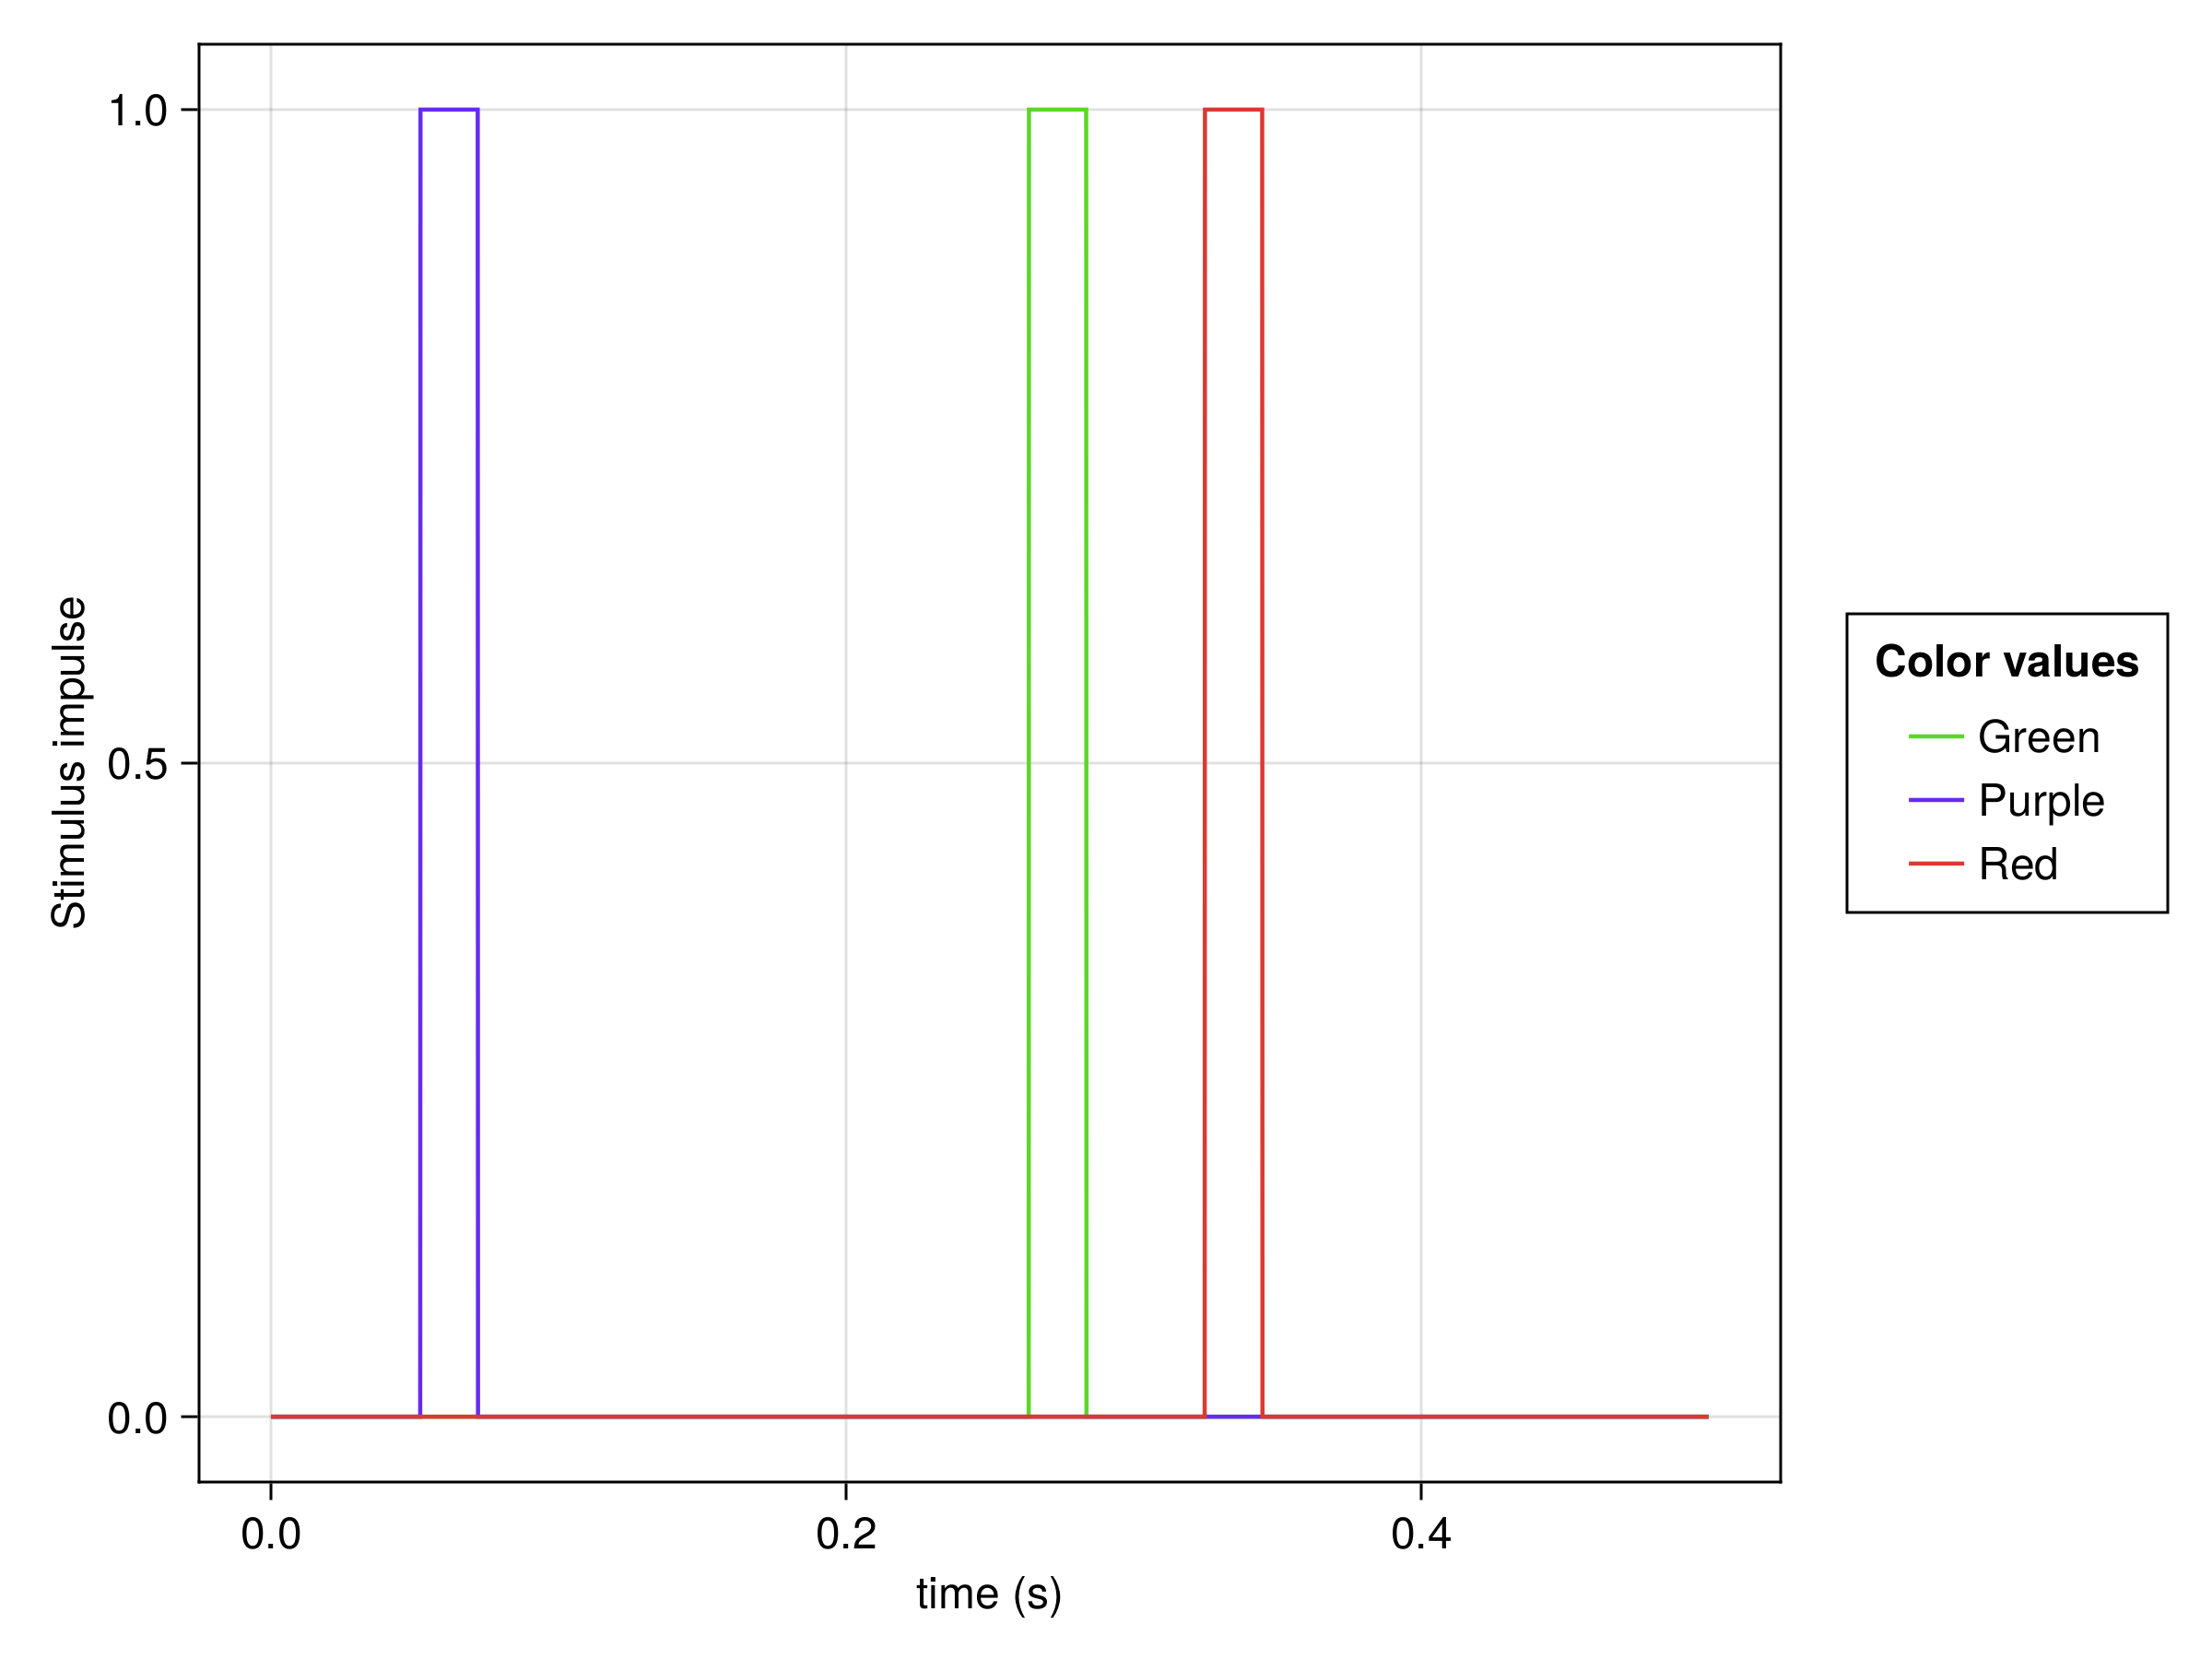
\includegraphics[scale=0.10]{example_trial.png}}
\caption{A sample trial showing the colors \textit{purple}, \textit{green}, and \textit{red} being presented. This trial constitutes a valid set.}
\label{trial}
\end{figure}

The model was trained on a training dataset of $540$ trials. The proportion of accepting to rejecting trials in the training dataset was $50\%$. $27$ trails were generated for the testing dataset, where each trial consisted of a distinct combination of presented colors. Trials were mini-batched during training into batches of $108$ trials.

\subsection{Model}
\label{ctrnnmodel}

We describe our model according to the framework proposed in \cite{richards2019deep}.

\textbf{Architecture:} The model was a continuous-time RNN identical to the networks used in\cite{sussillo2013opening,mante2013context,kay2022neural,pals2023trained,sussillo2015neural,cueva2018emergence}:
\begin{equation}
    \tau \dot{x}_i(t) = -x_i(t) + \sum^{N}_{k=1} J_{ik}r_k(t) + \sum^{N^{in}}_{k=1}B_{ik}u_k(t) + b_i + \eta_i(t)\label{rnnmodel}
\end{equation}
\begin{equation}
    r_i(t) = \tanh(x_i(t))
\end{equation}
\begin{equation}
    z(t) = \sum^{N}_{k=1}W_{k}r_k(t) + b_{out}
\end{equation}
$\tau$ is interpreted as the time constant for the RNN and was set to $10 ms$. $x_i(t)$ is interpreted as the average voltage of the $i$th subpopulation of neurons at time $t$. $N$ is the total number of subpopulations of neurons and was set at $100$. $u_k(t)$ is interpreted as the $k$th input stimulus conveying encoded color. $N^{in}$ is the number of input dimensions and was, as stated in sec.~\ref{taskmethod}, set at $100$. $\eta_i(t)$ is a random value drawn from a Gaussian distribution, $\mathcal{N}(0,0.10)$. $r_i(t)$ is interpreted as the average firing rate for the $i$th subpopulation of neurons. The activation function that converted average voltage to average firing rate is the hyperbolic tangent (tanh) function. $z(t)$ is interpreted as the average firing rate of the population of output neurons at time $t$.

Equation (\ref{rnnmodel}) was approximated with Euler's method using a step size ($\Delta t$) of $10 ms$ for all trials. The entirety of our model was coded in Julia\cite{bezanson2017julia} using the Lux framework\cite{pal2022lux} and SciML ecosystem\cite{rackauckas2017differentialequations,rackauckas2020universal}.

\textbf{Learning algorithm:} We used the AdamW learning algorithm\cite{loshchilov2017decoupled} and reverse mode automatic differentiation to update trainable parameters. The trainable parameters were the initial state $\textbf{x}(t=0)$, recurrent matrix $\textbf{J}$, input matrix $\textbf{B}$, recurrent bias $\textbf{b}$, output matrix $\textbf{W}$, and output bias $b_{out}$. The initial learning rate was set to $10^{-4}$. As referenced in sec.~\ref{interpretablemotifs}, an L2 regularization was imposed on the trainable parameters. We implemented this regularization through the AdamW learning algorithm with the weight decay parameter set to $10^{-4}$.

\textbf{Objective function:} We used a mean squared error (MSE) objective function to measure the difference between the observed $z(t)$ and the expected $\hat{z}(t)$. The last $50 ms$, corresponding to the last $5$ time steps, of $z(t)$ of each trial were measured against $\hat{z}(t)$. As referenced in sec.~\ref{interpretablemotifs}, an L2 regularization was imposed on the recurrent activations of the RNN. We implemented this regularization as an added term in the objective function. The full objective function was the following:
\begin{equation}
    \mathcal{L}(\hat{z},z,\textbf{r}) = \frac{1}{5}\sum_{t=T-5}^{T}(\hat{z}(t)-z(t))^2 + \frac{\lambda}{TN} \sum_{t,i=1}^{T,N} r^2_i(t)\Delta t
\end{equation}
$T$ is the total number of time steps across all trials and, via Euler's method, was set at $50$. $\lambda$ is the L2 regularization parameter and was set to $10^{-4}$.

\subsection{Analysis}
\label{analysismodel}

In order to interpret the learned dynamics of our model, we used principal component analysis (PCA). As a prevalent dimensionality reduction technique, PCA has been used in previous work to visualize and interpret the low-dimensional dynamics of RNNs\cite{sussillo2013opening,mante2013context,driscoll2022flexible,kay2022neural,pals2023trained}. In our study, we applied PCA to the firing rates of the RNN, $\textbf{r}(t)$, under conditions of no recurrent noise, $\eta_i(t)=0$. This approach enabled us to identify potential dynamical mechanisms.

However, it is crucial to recognize that PCA primarily uncovers the strongest correlations among the firing rates of the RNN rather than elucidating causal, mechanistic properties of the entire model\cite{langdon2022latent}. To address this inherent limitation of PCA, we supplemented our analysis by developing a simplified model. This model, guided by insights from PCA, emulated the dynamics of the RNN and served to verify the mechanisms suggested by our PCA-based interpretation. This combination of methods strengthens the validity of our findings.

\section{Hypothesis}

Our initial hypothesis posited that PCA would reveal that our trained model learned a low-dimensional network comprised of attractive fixed points. We hypothesized that the model's dynamics would originate from a central attractor within this network and the presentation of encoded colors would then transition these dynamics towards surrounding attractors. At the end of the trial, the final attractor that the dynamics settled into would have an associated classification label of either a valid or an invalid set (Fig.~\ref{hypothesisFSA}).

\begin{figure}[htbp]
\centerline{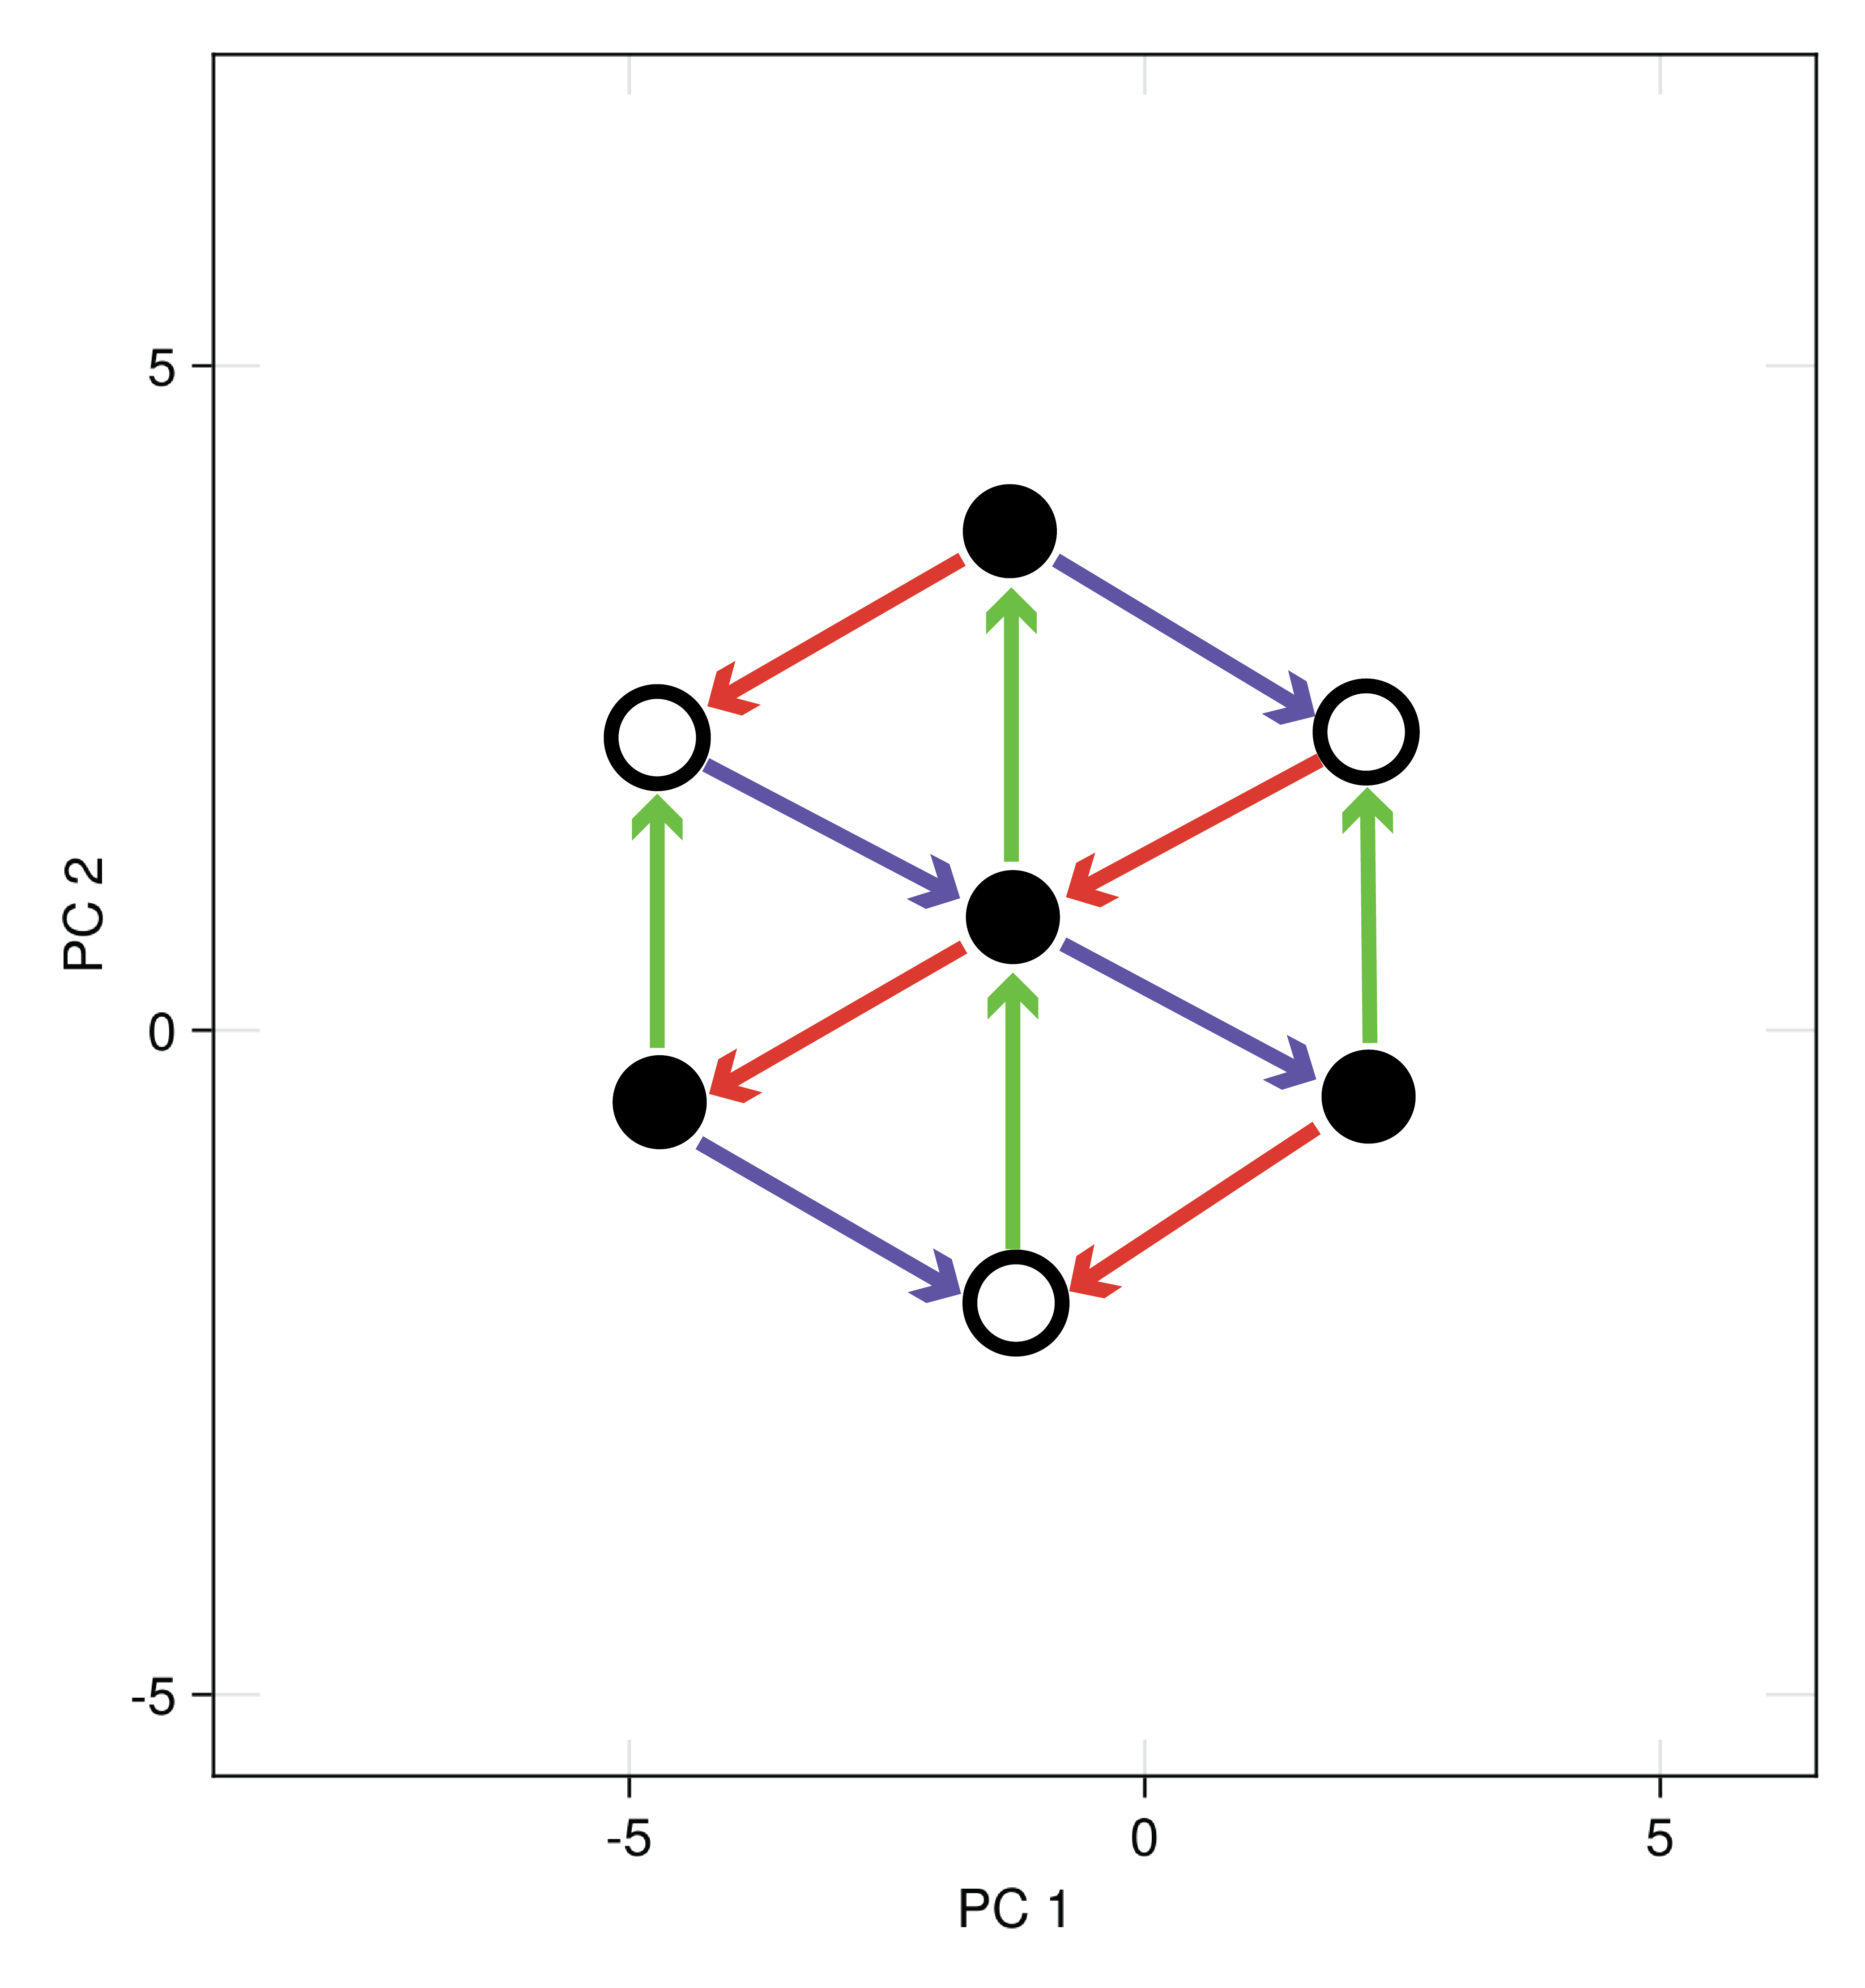
\includegraphics[scale=0.15]{hypothesis.png}}
\caption{Our hypothesized dynamical mechanism. Each circle is an attractive fixed point. Filled circles denote attractors classified as a valid set. Empty circles denote attractors classified as an invalid set. The model's dynamics begin in the central attractor. Our first and second assumption resulted in a hexagonal tiling of the networks fixed points.}
\label{hypothesisFSA}
\end{figure}

This hypothesis was predicated on two fundamental assumptions:
\begin{enumerate}
\item The model's dynamics would exhibit attraction.
\item Presented colors would be linearly encoded into the model's dynamics.
\end{enumerate}
The first assumption drew inspiration from the Hopfield network\cite{hopfield1982neural}, where memories are stored as attractive fixed points. Unlike the Hopfield network, which only receives stimuli at the onset of its dynamics, our hypothesis takes into account a sequential presentation of colors as required by our task. Despite this difference, the Hopfield network's central insight---that memories in a neural circuit can be encoded with attractive dynamics---has found validation in experimental work\cite{chaisangmongkon2017computing,khona2022attractor}. Therefore, we integrated this concept of attractive dynamics into our hypothesized dynamical mechanism.

The second assumption was influenced by a variety of computational studies that demonstrated the crucial role linear encoding of stimuli can play in shaping an RNN's learned dynamical mechanism\cite{sussillo2013opening,mante2013context,driscoll2022flexible,kay2022neural}. Furthermore, given that the input matrix $\textbf{B}$ in equation (\ref{rnnmodel}) is not a function of time, voltage, or firing rate, we assumed that the presentation of a color at any point in the dynamics should result in a linear perturbation of the same magnitude and direction as a presentation of the same color at any other point in the dynamics. Thus, our hypothesis adopted this linear encoding of colors as a fundamental assumption.

We further noticed that this hypothesis of transitions between attractors in a network of fixed points closely resembles the transitions between states in an FSA. Previous work has drawn the analogy between RNNs and FSA before\cite{cleeremans1989finite}, and in this study, we sought to further build on this analogy in the context of low-dimensional dynamical mechanisms.

\section{Results}

\subsection{Training and testing accuracy}

The fully-trained RNN model demonstrated robust performance, achieving an accuracy of $96.30\%$ on training data and $100.00\%$ on testing data. In the absence of recurrent noise, the model achieved perfect accuracy, reaching an accuracy of $100.00\%$ on both training and testing data. This perfect accuracy was expected due to the algorithmic nature of the task\cite{power2022grokking,nanda2023progress}. 

Throughout a trial, the model's output, $z(t)$, exhibited a large oscillation with \textit{perturbations} corresponding to the presentation of encoded colors (Fig.~\ref{exampletrialstimuli}). To recognize valid sets, the output's oscillation ended the trial in the positive phase, yielding a value of $+1$. Conversely, to recognize invalid sets, the output's oscillation ended the trial in the negative phase, yielding a value of $-1$. In the absence of encoded color input, the model completes two full oscillations. The \textit{perturbations} corresponding to color presentation indicated some influence on the oscillation, yet the computational significance remained unclear without further analysis.

\begin{figure}[htbp]
\centerline{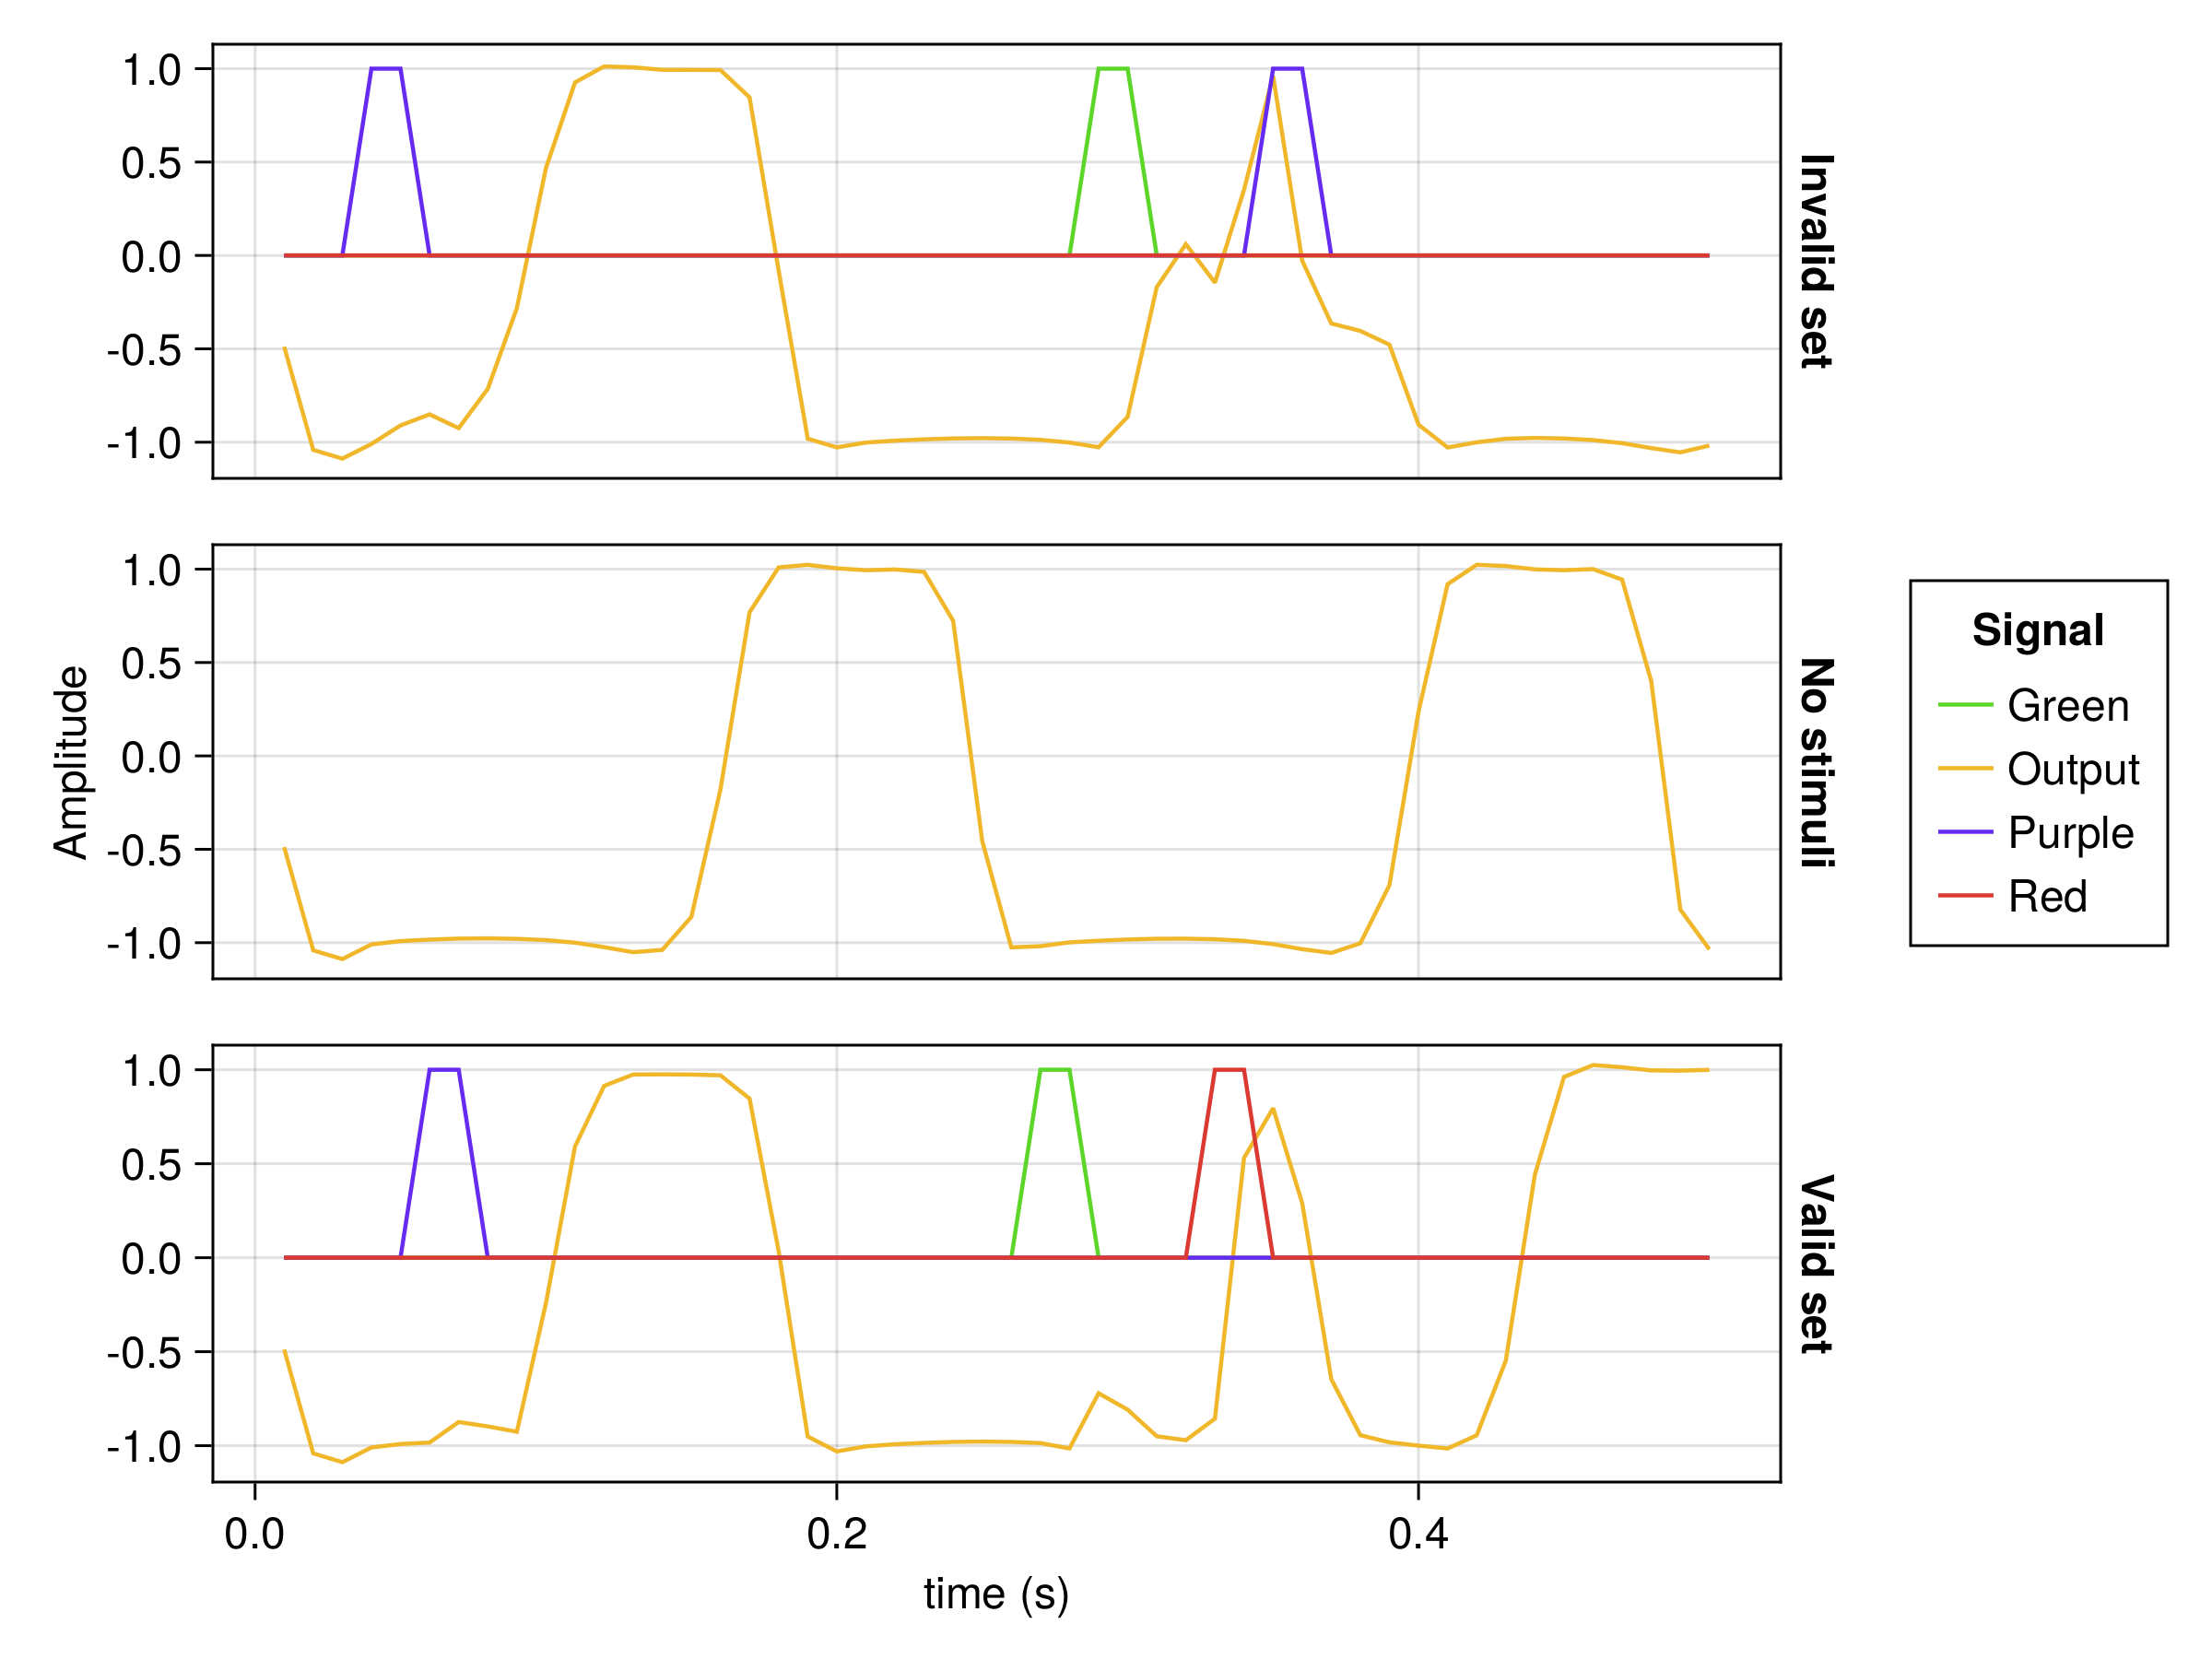
\includegraphics[scale=0.10]{SET_examples.png}}
\caption{Three examples of trials and the resulting model output. The top row displays a trial with an invalid set and the resulting model output of $-1$. The middle row displays a trial with no presented colors and demonstrates the model output completing two full oscillations. The bottom row displays a trial with a valid set and the resulting model output of $-1$. Note the \textit{perturbations} caused by the presentation of colors in the top and bottom rows.}
\label{exampletrialstimuli}
\end{figure}

\subsection{PCA insights}

PCA revealed that the model learned a low-dimensional limit cycle\footnote{Refer to \cite{strogatz2018nonlinear} for an overview of limit cycles in nonlinear dynamics.} which completed two full rotations during a trial (Fig.~\ref{pcasummary}). At the end of the trial, PCA revealed that the dynamics of the model would lie in one of three distinct distributions along the limit cycle. Two distributions corresponded to invalid sets and one distribution corresponded to valid sets. These findings indicated that the presentation of colors would shift the phase of the limit cycle. We inferred this phase shift to be the computational affect of the \textit{perturbations} seen in Fig.~\ref{exampletrialstimuli}.

\begin{figure}[htbp]
\centerline{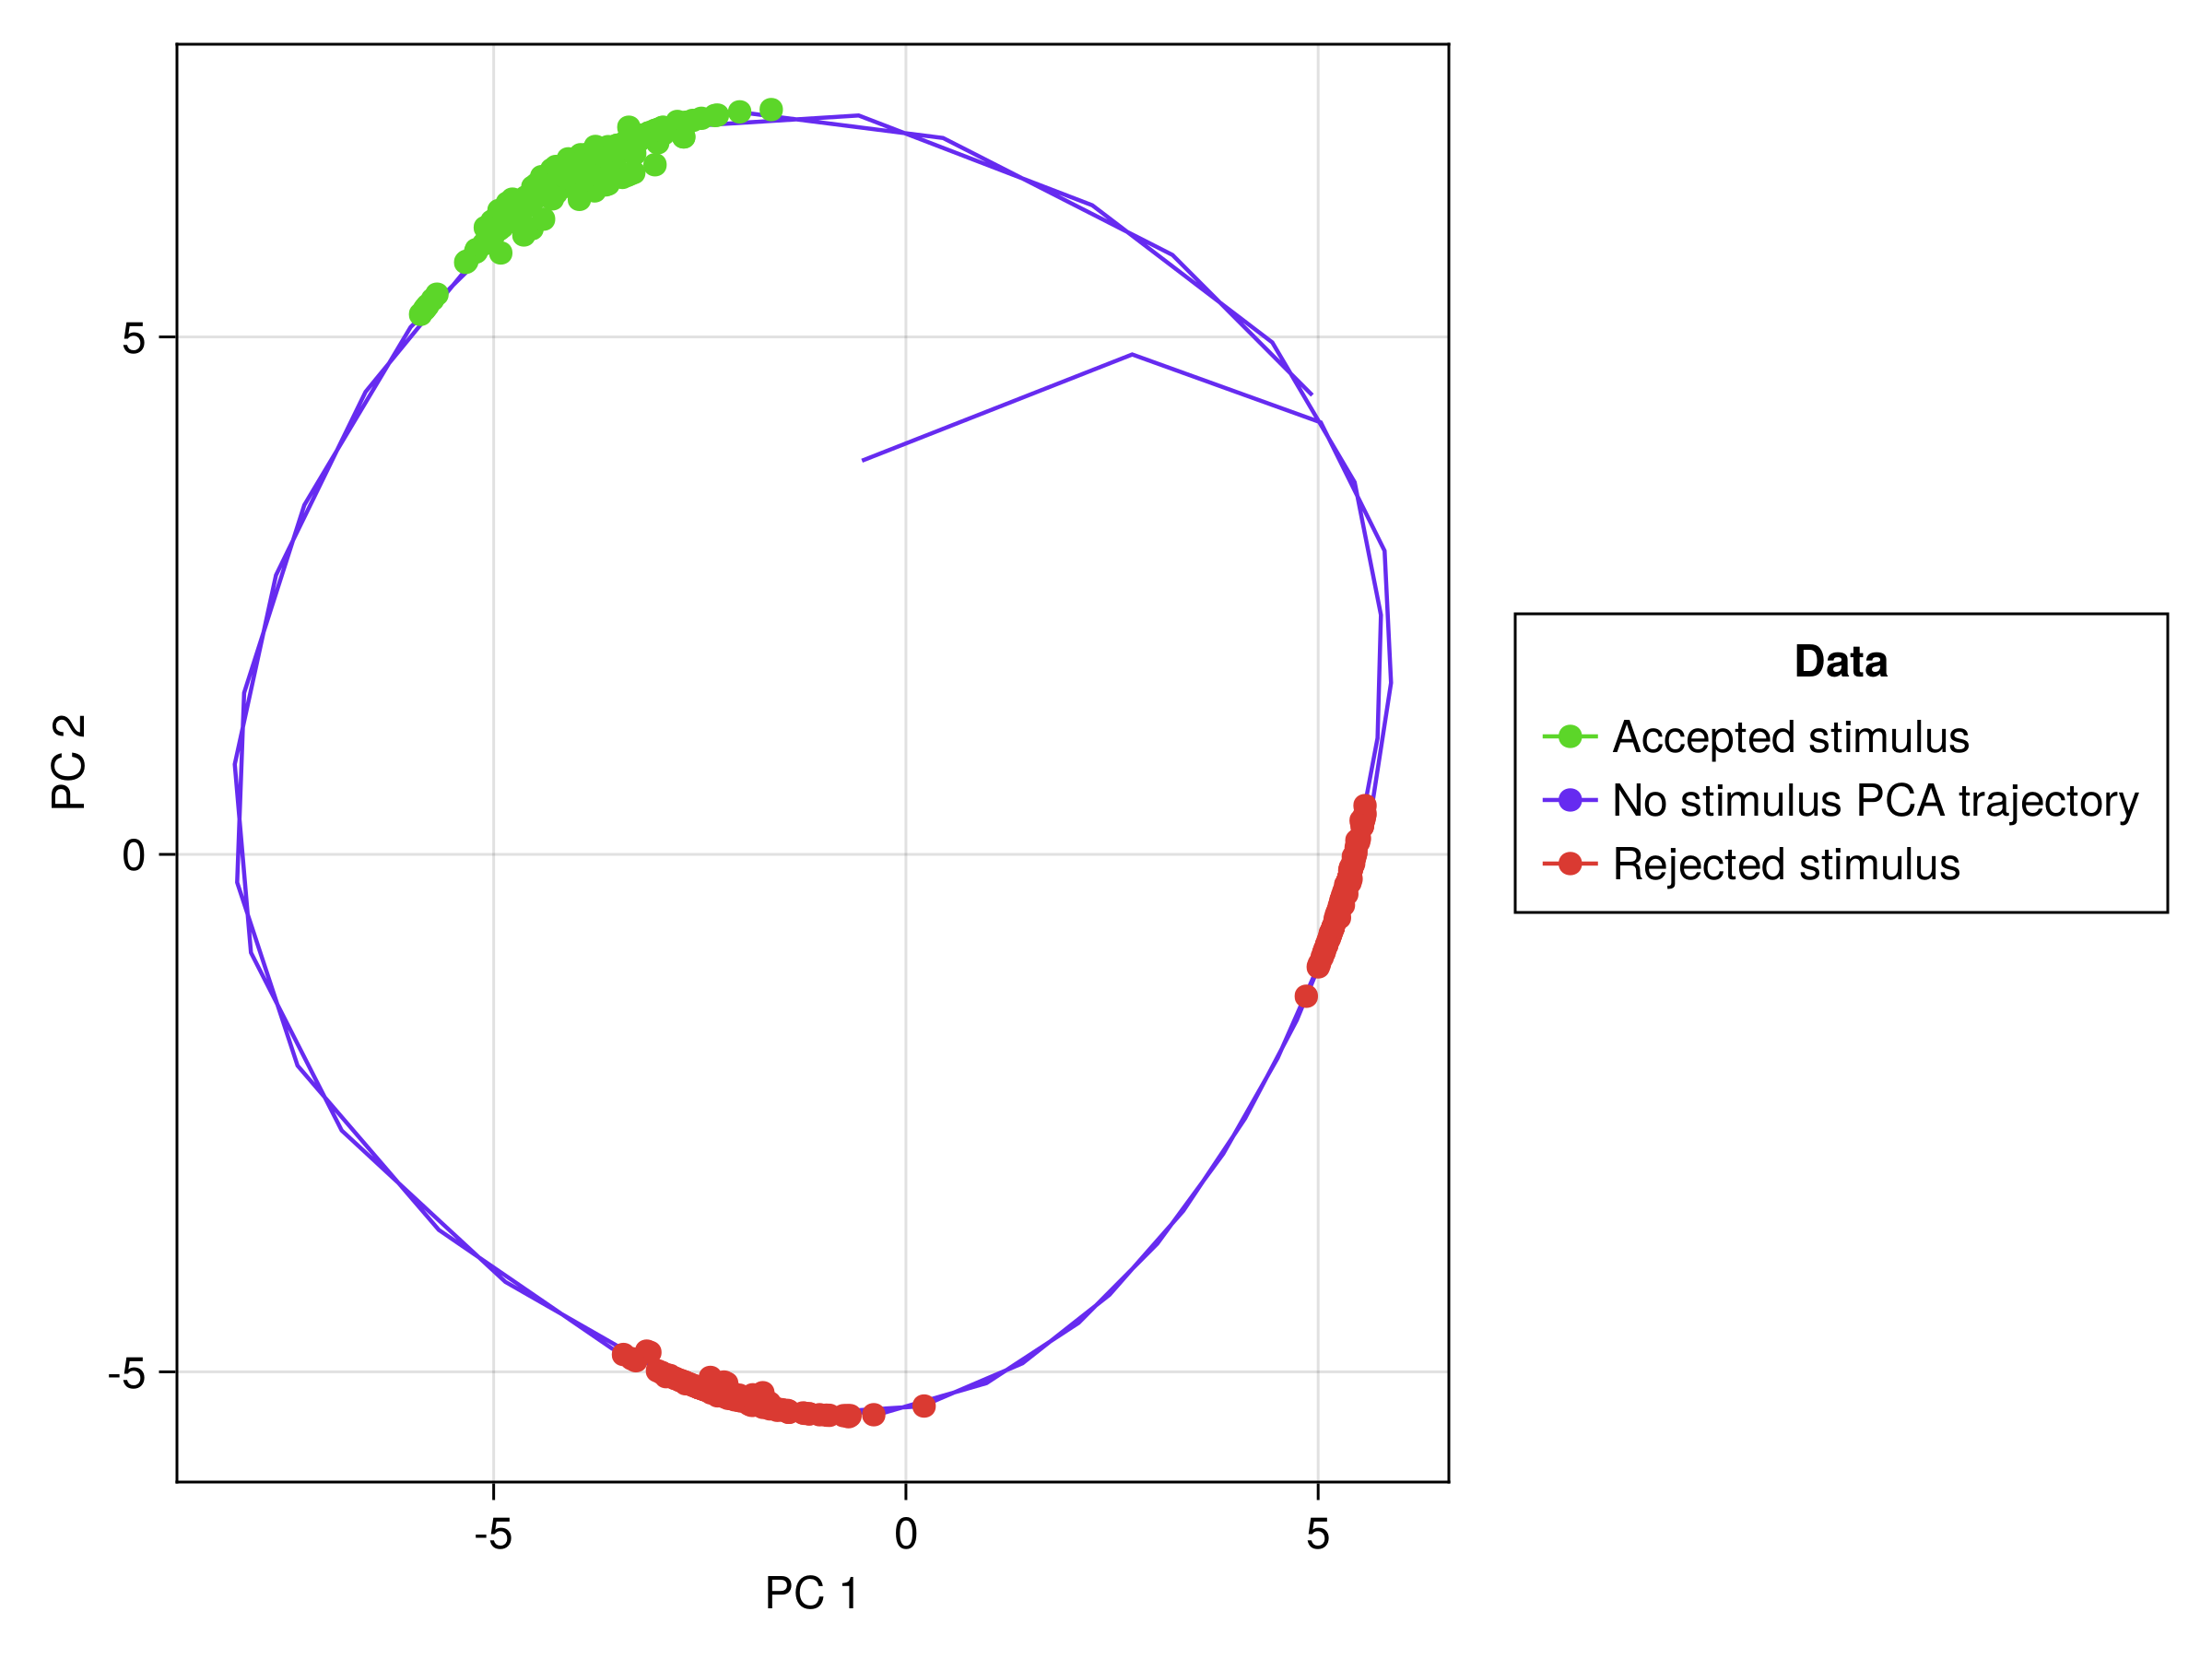
\includegraphics[scale=0.10]{pca_summary.png}}
\caption{The model's dynamics projected onto PC 1 and PC 2. The purple trajectory is the projected dynamics of the model during a trial with no stimulus. The green points are the endpoints of the model’s dynamics during trials with valid sets. The red points are the endpoints of the model’s dynamics during trials with invalid sets.}
\label{pcasummary}
\end{figure}

In order to confirm that the presentation of colors led to phase shifts in the model's limit cycle, we rotated PCA trajectories and examined the resulting oscillations. This rotation was conducted due to the observation that projecting the model's dynamics entirely onto principal component (PC) 1 would lead to a mixing of distributions corresponding to valid and invalid sets. Through a $60$-degree rotation, the distributions corresponding to valid and invalid sets became maximally separable when projected onto rotated principal component (rPC) 1.

Fig.~\ref{pcaacceptedsets} illustrates the model's dynamics projected onto rPC 1 over time for various trials. By examining the influence of presented colors on the dynamics across different trials, we developed hypotheses about the mechanistic effects of presented colors on the underlying limit cycle. \textit{Green} appeared to slightly perturb the model's dynamics, \textit{purple} appeared to rush the model's dynamics, and \textit{red} appeared to reset the model's dynamics.

\begin{figure}[htbp]
\centerline{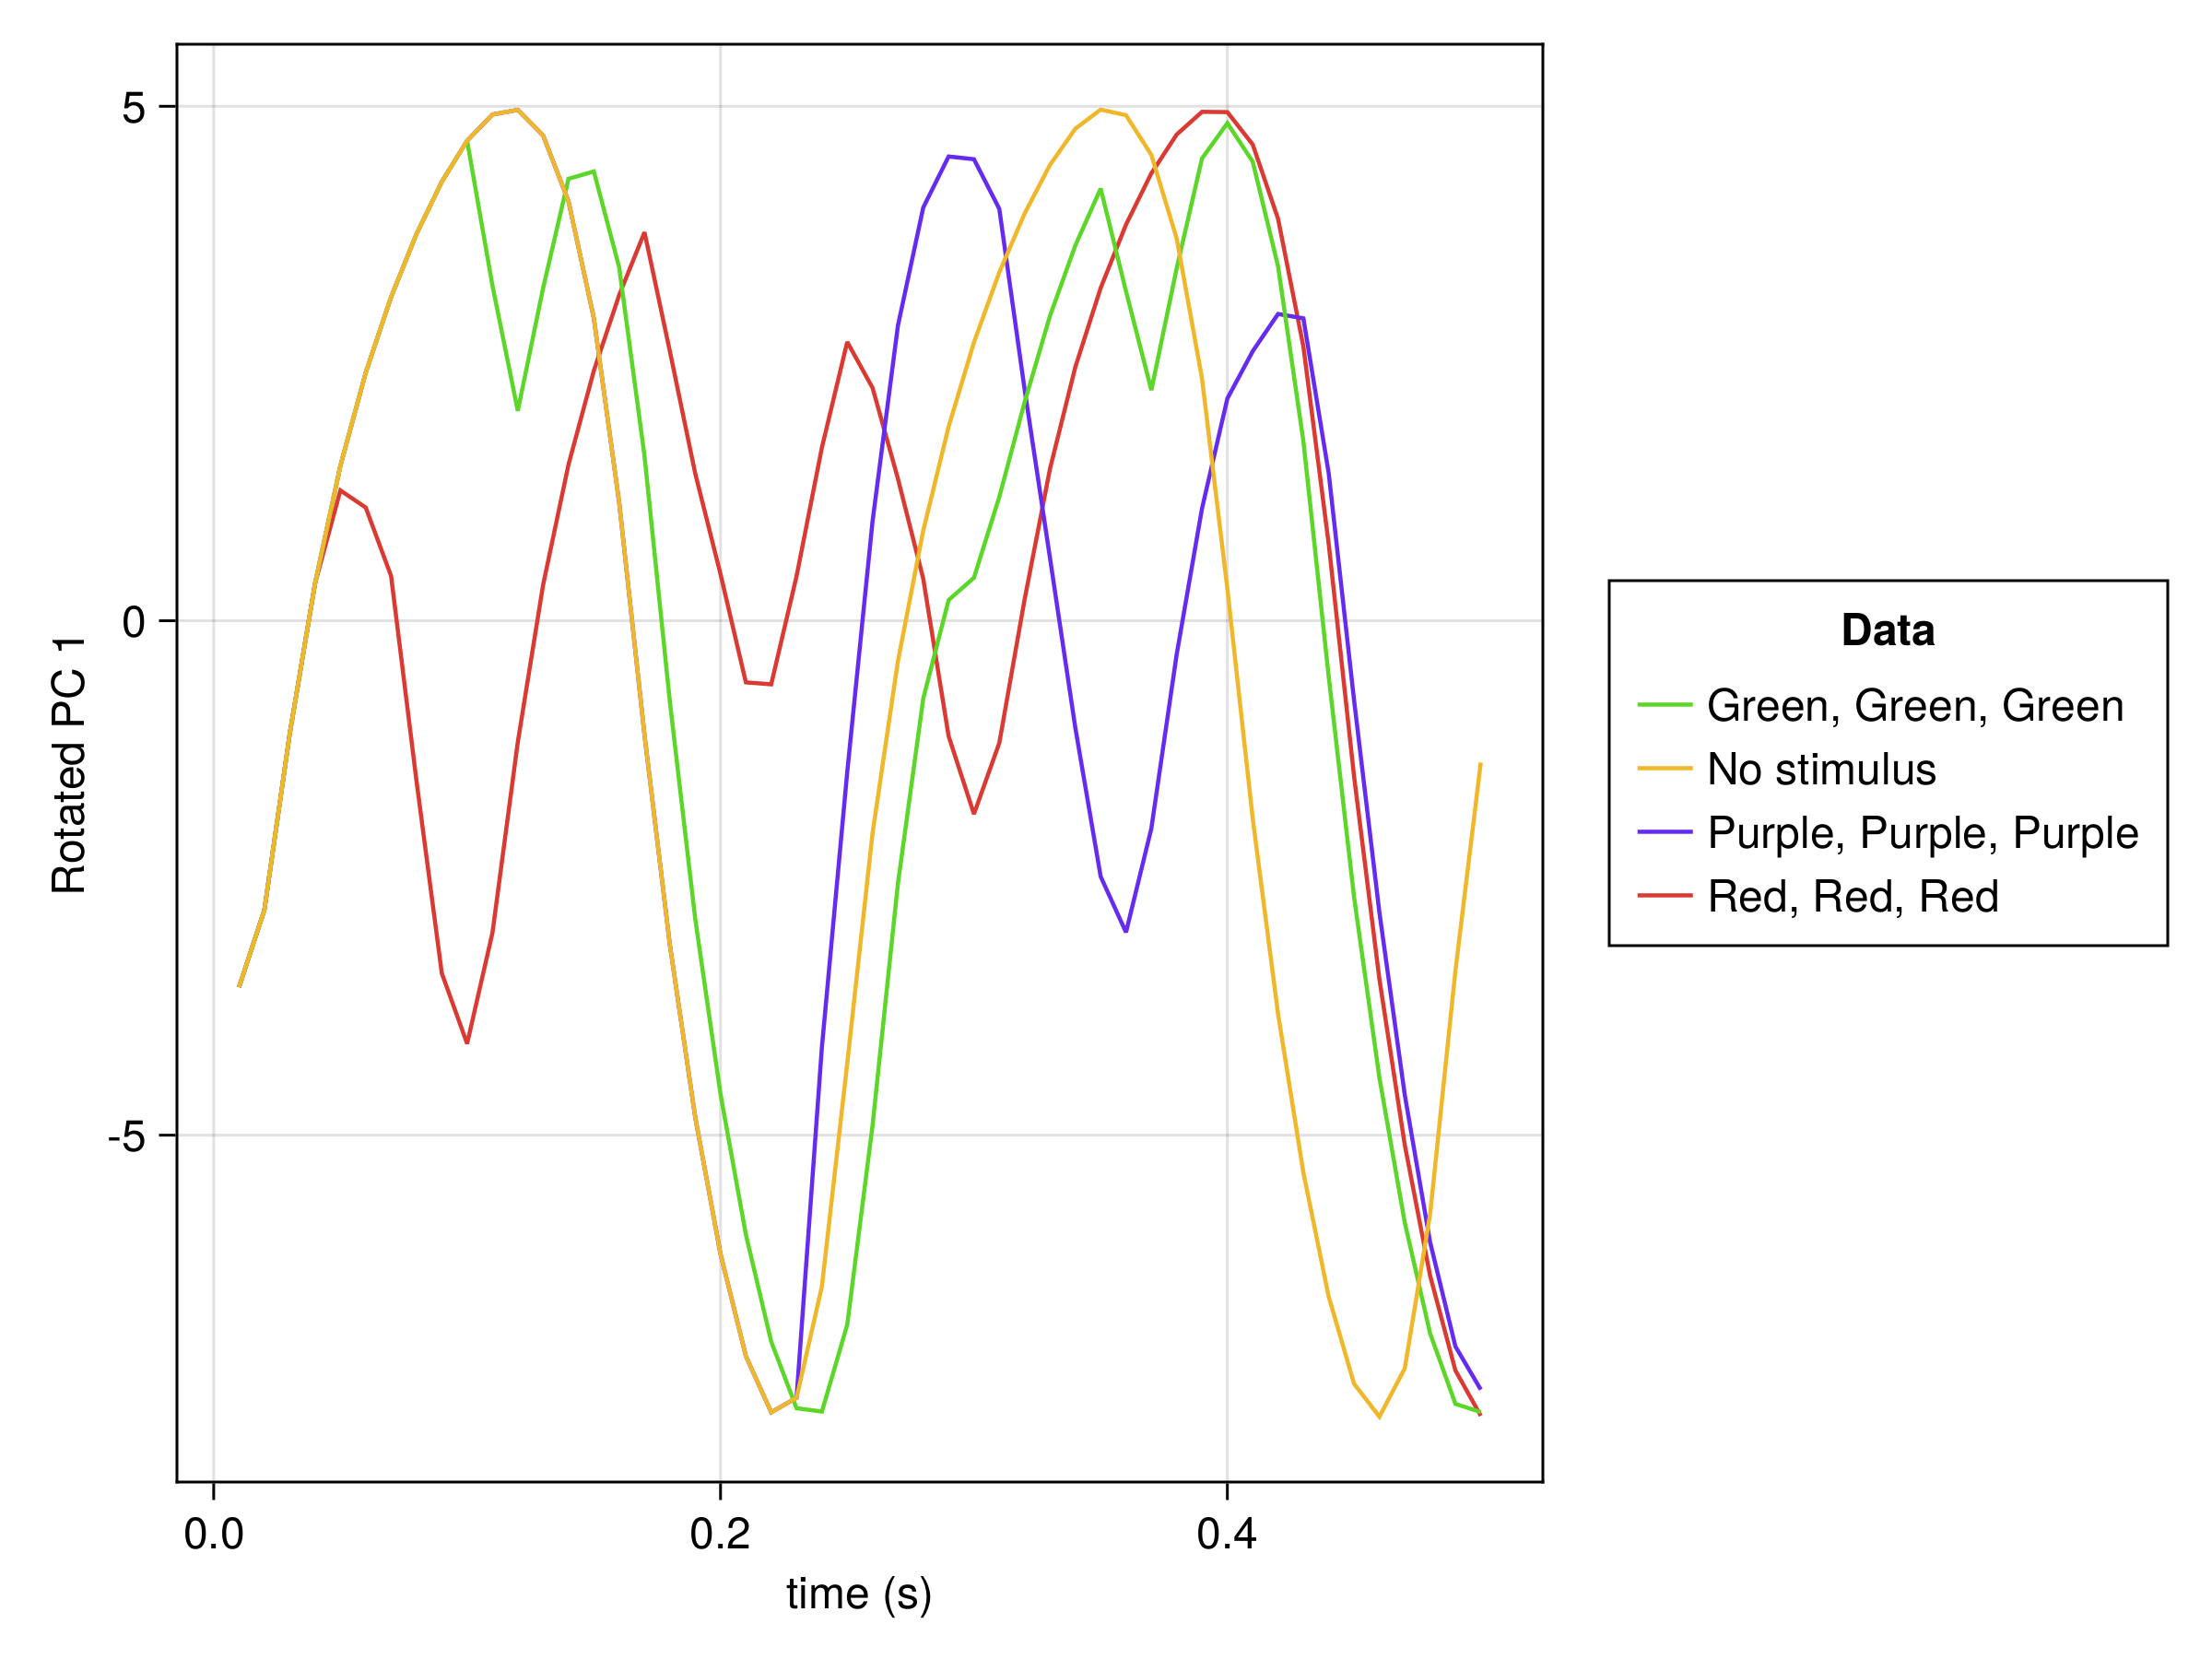
\includegraphics[scale=0.10]{rotated_pc1_accepted.png}}
\caption{The model’s dynamics projected onto rPC 1 for various trials. In the trial with no stimuli, the dynamics performed two complete oscillations. In the all-\textit{green} trial, the dynamics were minimally perturbed. In the all-\textit{purple} trial, the presentation of the color seemed to shift the phase of the limit cycle forward. In the all-\textit{red} trial, the color presentation appeared to shift the phase backward.}
\label{pcaacceptedsets}
\end{figure}

Contrary to our initial hypothesis—which suggested that the model would learn a dynamical mechanism characterized by attractive fixed points and a linear encoding of colors—the oscillatory dynamics of both the output (Fig.~\ref{exampletrialstimuli}) and the PCA trajectories (Fig.~\ref{pcasummary} and Fig.~\ref{pcaacceptedsets}) led us to reconsider our fundamental assumptions. Instead, we discovered that the model learned a dynamical mechanism characterized by phase shifts in a limit cycle. Remarkably, the analogy to an FSA persisted with this new dynamical mechanism. Rather than the FSA residing in the state space of the dynamics, it now exists in the phase angle state space of the limit cycle with phase shifts analogous to state transitions (Fig.~\ref{resultingfsa}).

\begin{figure}[htbp]
\centerline{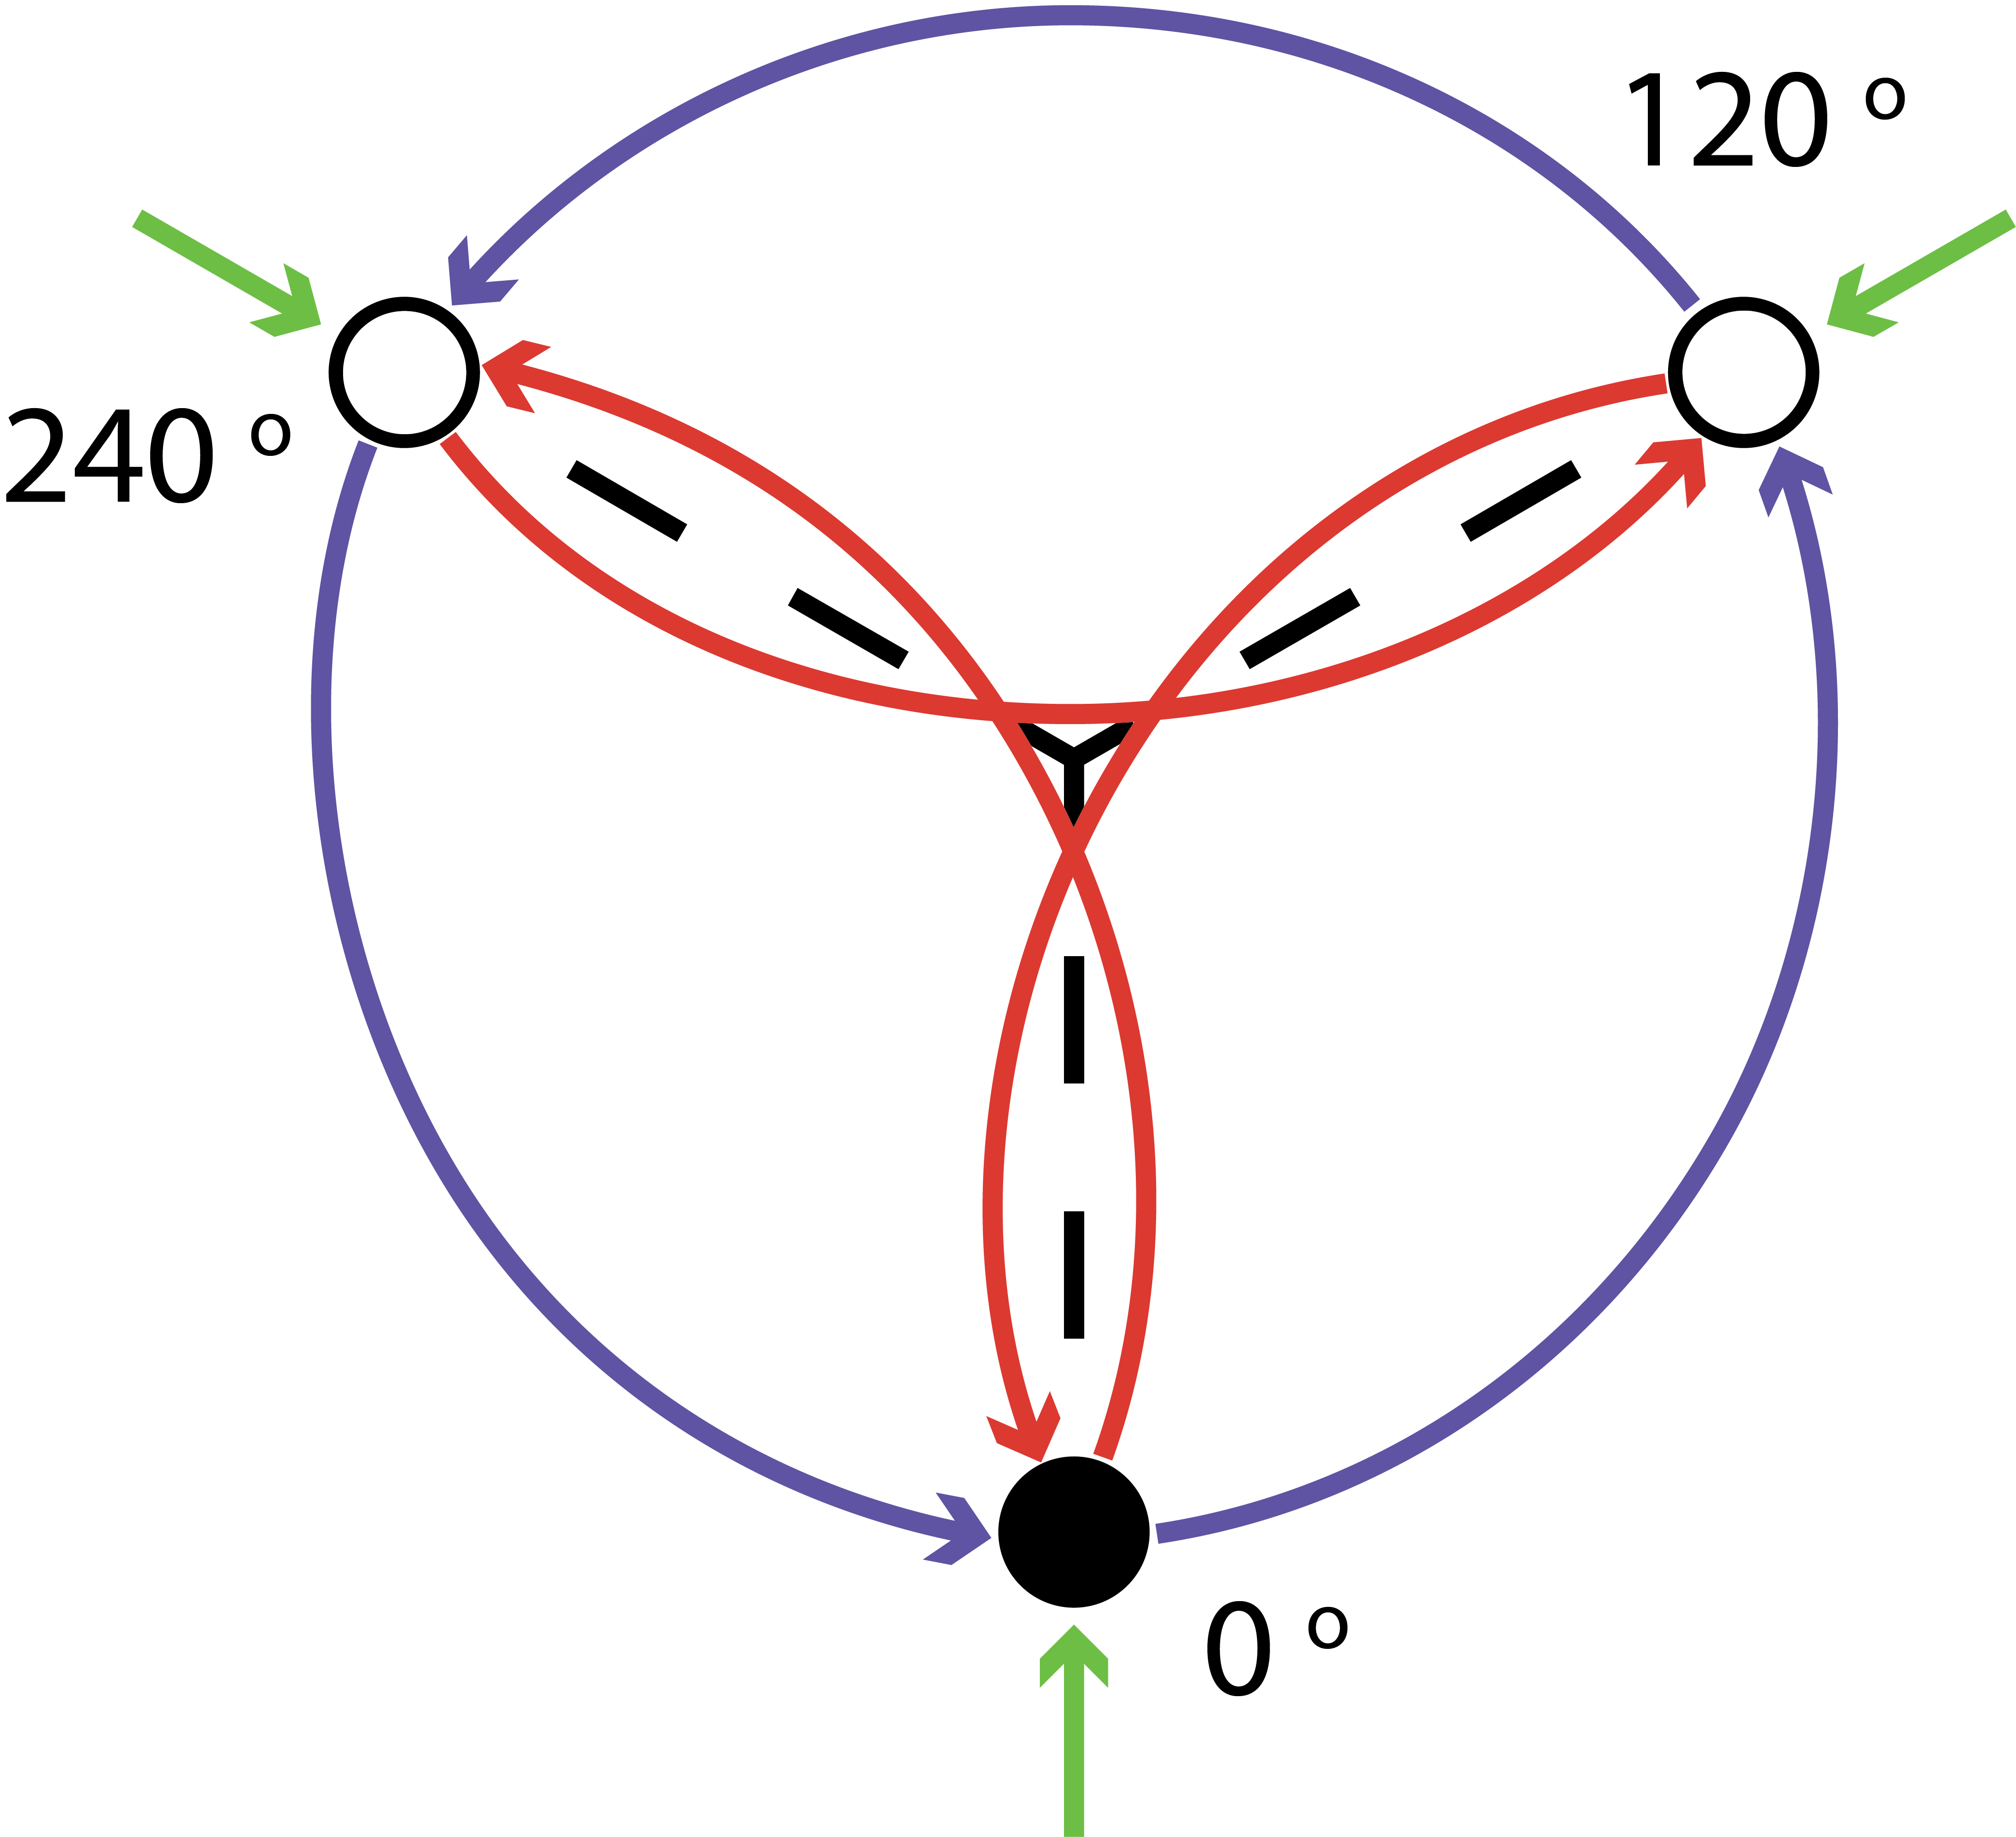
\includegraphics[scale=0.125]{resulting_FSA.png}}
\caption{The learned FSA exists in the phase angle state space of the limit cycle. The automaton starts at a phase angle of $0$ degrees and the presentation of colors causes transitions to other states, each representing a distinct phase angle in the limit cycle.}
\label{resultingfsa}
\end{figure}

While we previously observed that the presentation of the color \textit{green} did impact the model's dynamics (Fig.~\ref{pcaacceptedsets}), we interpreted the learned dynamical mechanism under the assumption that \textit{green} did not impact the dynamics in order to simplify the FSA analogy (Fig.~\ref{resultingfsa}). We interpreted \textit{purple} as adding $120^o$ to the phase angle and \textit{red} as subtracting $120^{\circ}$. Hence, it becomes clear how presenting all the \textit{same} or \textit{different} colors would cause the limit cycle's phase shifts to sum to $0^{\circ}$, $360^{\circ}$, or $-360^{\circ}$ and cause the model's output to end the trial in the valid set phase.

To test the accuracy of our interpreted dynamical mechanism, we made predictions about the ending phase of the model's dynamics when projected onto rPC 1 in trials with invalid sets. For example, if the sequence of presented colors is \textit{purple}, \textit{green}, \textit{purple}, the model should end $120^{\circ}$ behind the valid set phase. Conversely, if the sequence of presented colors is \textit{red}, \textit{green}, \textit{red}, the model should end $120^{\circ}$ ahead of the valid set phase. Fig.~\ref{pcarejectedsets} supports these predictions and our interpretation of the learned dynamical mechanism.

\begin{figure}[htbp]
\centerline{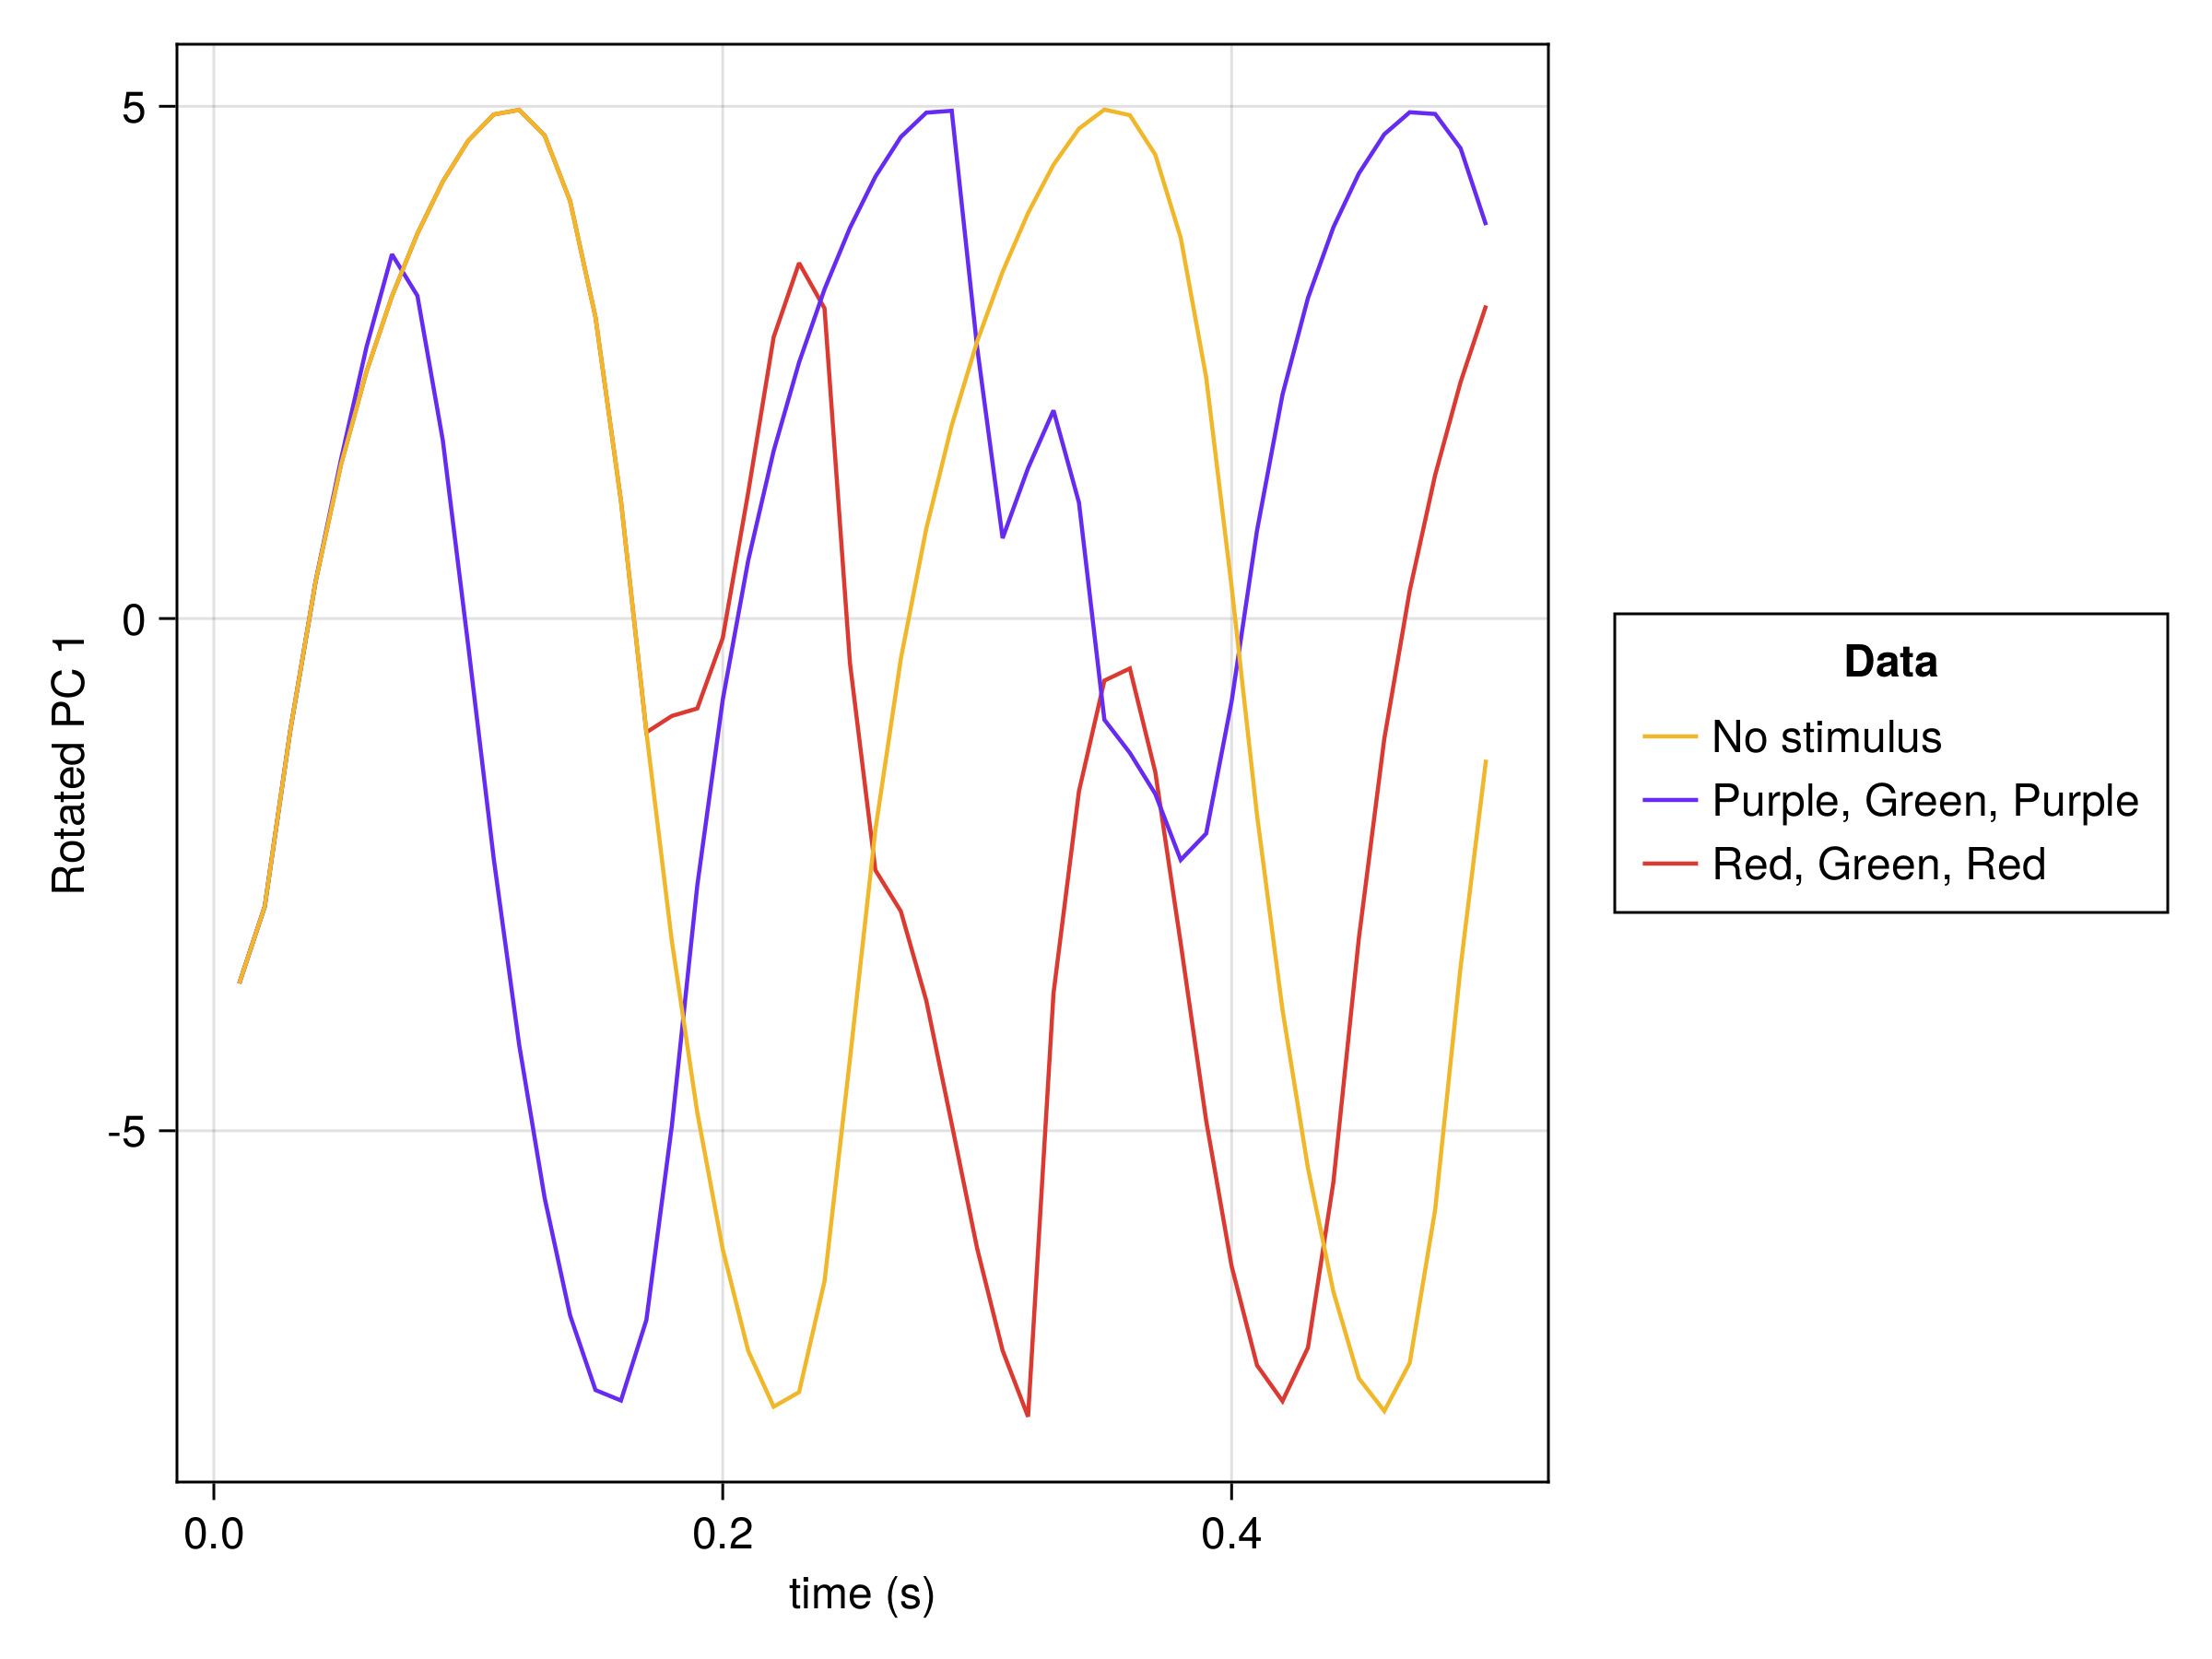
\includegraphics[scale=0.10]{rotated_pc1_rejected.png}}
\caption{The ending phase of rPC 1 for trials of invalid sets supports our interpretation of the learned dynamical mechanism. A \textit{purple}, \textit{green}, \textit{purple} trial results in rPC 1 ending $120^{\circ}$ behind the valid set phase. A \textit{red}, \textit{green}, \textit{red} trial results in rPC 1 ending $120^{\circ}$ ahead of the valid set phase.}
\label{pcarejectedsets}
\end{figure}

\subsection{Handcrafting an oscillatory model}

To further validate our interpretation of the learned dynamical mechanism and its analogy with FSA, we designed a simple oscillatory model to emulate the dynamics of our trained model. Specifically, we handcrafted the following equation to reproduce the projection of our model's dynamics onto rPC 1:
\begin{equation}
f(t) = 7\sin (\frac{2\pi}{0.29}t+\int_{0}^{t}\phi(\tau)\,d\tau)-1.5\label{simpmodel}
\end{equation}
$\phi(\tau)$ corresponds to the presentation of an encoded color: if \textit{purple} is presented at time $\tau$, then $\phi(\tau)=\frac{2\pi}{3}$; if \textit{red} is presented, then $\phi(\tau)=-\frac{2\pi}{3}$; and if \textit{green} or no color is presented, then $\phi(\tau)=0$.

It is worth noting that equation (\ref{simpmodel}) simplifies many of the dynamical properties observed in rPC 1. For instance, the frequency of the dynamics was nonuniform (Fig.~\ref{pcasummary}) and color presentation caused complex perturbations in the model’s dynamics (Fig.~\ref{pcaacceptedsets}). However, equation (\ref{simpmodel}) models the frequency as constant at $\frac{2\pi}{0.29}$ and models color presentation as causing simple perturbations by integration. Despite these simplifications, equation (\ref{simpmodel}) qualitatively captures the model’s dynamics projected onto rPC 1 (Fig.~\ref{constructedmodel}). The similarity between the dynamics of our trained model and our handcrafted model further supports our interpretation of the learned dynamical mechanism.

\begin{figure}[htbp]
\centerline{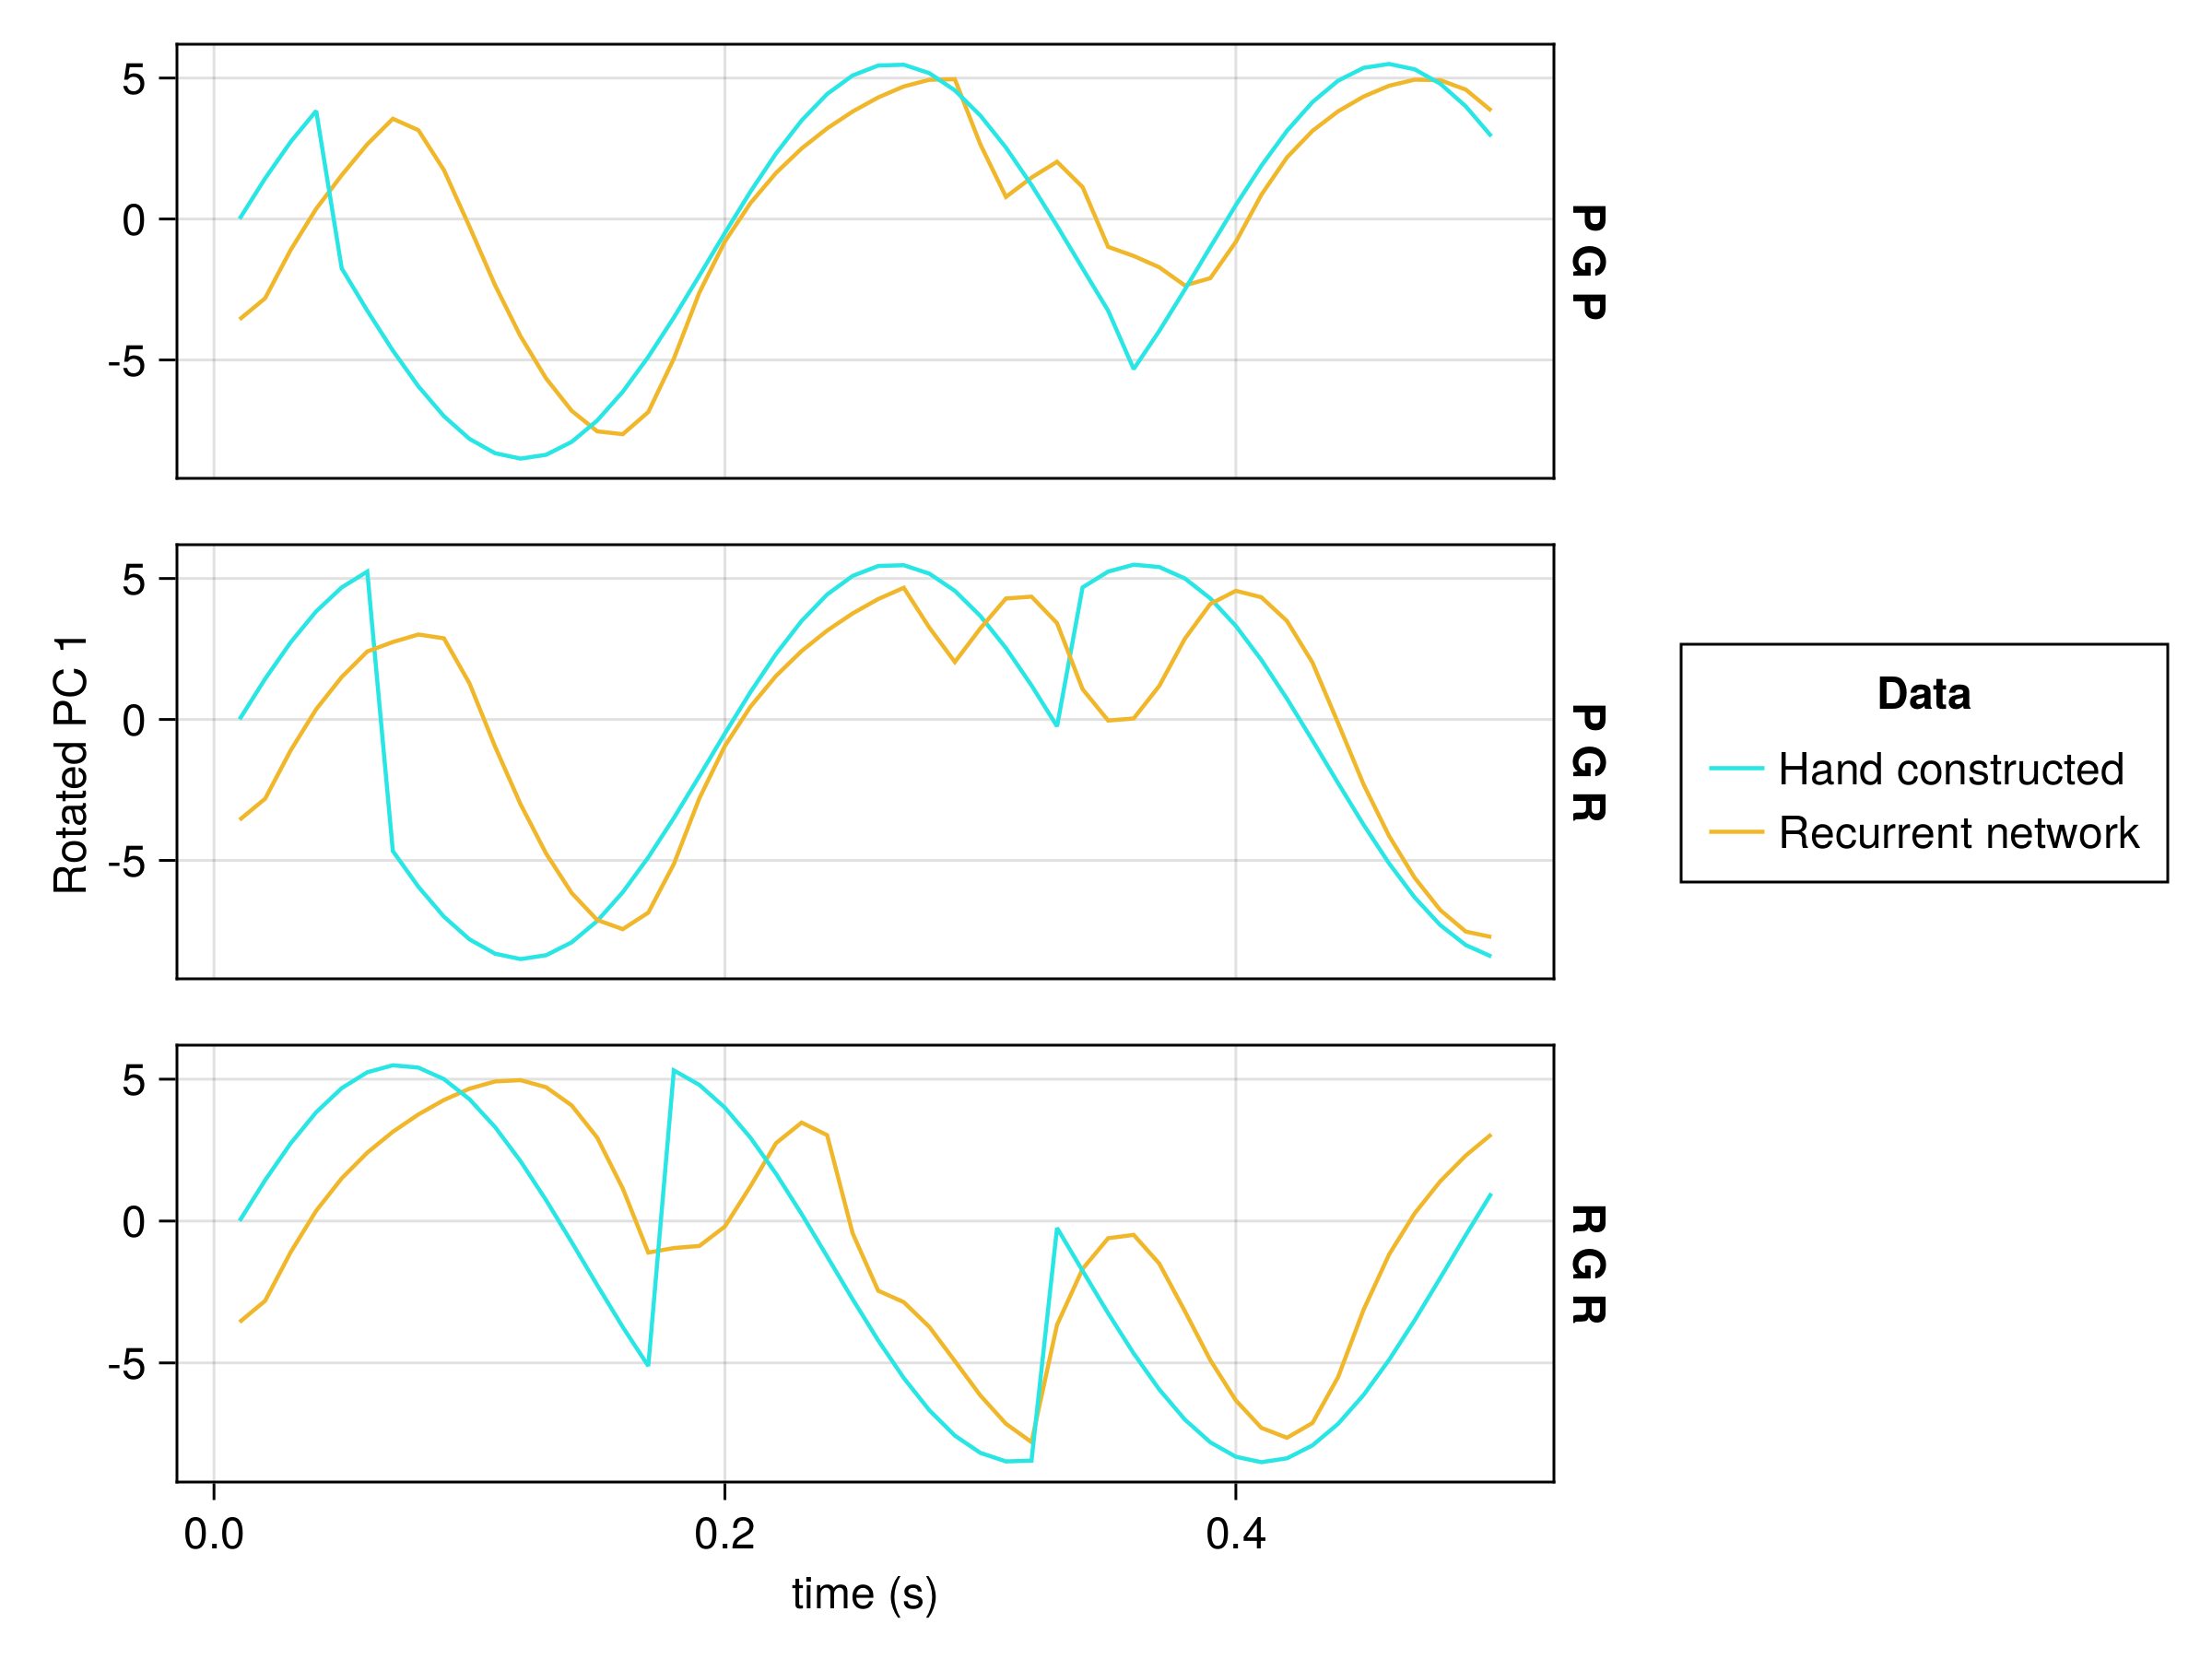
\includegraphics[scale=0.10]{constructed_phase_angle_computation.png}}
\caption{Our handcrafted oscillatory model qualitatively captures our trained model’s dynamics projected onto rPC 1. The top row shows model dynamics in a \textit{purple}, \textit{green}, \textit{purple} trial. The middle row shows model dynamics in a \textit{purple}, \textit{green}, \textit{red} trial. The bottom row shows model dynamics in a \textit{red}, \textit{green}, \textit{red} trial.}
\label{constructedmodel}
\end{figure}

\section{Discussion}

In this study, we demonstrated how an RNN, trained on a simple pattern recognition task inspired by the SET card game, could recognize patterns via phase shifts in a limit cycle. We employed PCA to identify three distinct distributions of endpoints in our model's dynamics, each corresponding to a distinct phase angle in the limit cycle (Fig.~\ref{pcasummary}), and showed how the presentation of colors caused transitions between these phase angles (Fig.~\ref{pcaacceptedsets}). Additionally, we drew an analogy between phase shifts in the limit cycle and state transitions in an FSA (Fig.~\ref{resultingfsa}). The validity of our interpretation of the learned dynamical mechanism, as well as the FSA analogy, was strengthened by the prediction of the ending phase of our model's dynamics (Fig.~\ref{pcarejectedsets}) and the construction of a handcrafted oscillatory model that mimicked these dynamics (Fig.~\ref{constructedmodel}). In essence, we have developed a robust narrative detailing the learned dynamical mechanism of an RNN trained on a simple pattern recognition task.

Interestingly, the dynamical mechanism learned in our study challenged two fundamental assumptions pertaining to our original hypothesis, specifically that the model would learn attractive dynamics and linearly encode colors. Although there are theoretical\cite{hoppensteadt1999oscillatory} and computational\cite{kay2022neural,pals2023trained} precedents for oscillatory dynamics in RNNs, it remains unclear why our model opted for a mechanism characterized by oscillatory dynamics rather than attractive dynamics. Given the universal function approximation capabilities of RNNs\cite{funahashi1993approximation}, it is theoretically possible to for an RNN to learn a dynamical mechanism similar to our initial hypothesis. Perhaps by fine-tuning various model and task-related hyperparameters, we could bias our model towards learning attractive dynamics\cite{schaeffer2022no}.

Furthermore, the cognitive plausibility of FSA deserves further exploration. While FSA are simple computational models with deep roots in cognitive science\cite{chomsky1957syntactic}, the simplicity of our task and stimuli likely contributed to the emergence of an FSA-like dynamical mechanism. Introducing more complex stimuli and tasks might disrupt this FSA analogy, but it's also possible that the underlying algorithm our model might implement is represented by an FSA employing the dynamical mechanism elucidated in this study.

Looking ahead, it would be valuable to investigate how the mechanism uncovered here could integrate with other dynamical mechanisms to enable more complex computations. In particular, we are interested in how our dynamical mechanism might be integrated into the dynamics of an RNN trained on a full game of SET complete with visual search across all 12 cards\cite{gordon2017joy}. Ultimately, this line of research could lead toward constructing a dynamical computer capable of programming in a manner similar to conventional digital computers\cite{jaeger2021towards}.

Lastly, our findings and methodologies may have meaningful implications for mechanistic interpretability in the field of deep learning. This domain is focused on constructing mechanistic models of the learned computations of deep learning models with the aim to elucidate phenomena related to generalization and adversarial attacks\cite{power2022grokking,nanda2023progress}. Our work aligns with this research direction and the approaches used may prove valuable for future interpretability studies.

\section*{Acknowledgments}

We would like to thank Sabrina Drammis, Joshua Liu, Nancy Lynch, Nikasha Patel, and Brabeeba Wang for helpful discussions pertaining to the conceptualization of this work. We also acknowledge the assistance of OpenAI's ChatGPT in editing portions of this manuscript.

\begin{thebibliography}{00}
\bibitem{inhelder1964early} B. Inhelder and J. Piaget, \textit{The Early Growth of Logic in the Child: Classification and Seriation}. New York: Harper and Row, 1964.
\bibitem{bishop2006pattern} C. M. Bishop, \textit{Pattern Recognition and Machine Learning}. New York: Springer, 2006.
\bibitem{lecun2015deep} Y. LeCun, Y. Bengio, and G. Hinton, ``Deep learning,'' \textit{Nature}, vol. 521, no. 7553, pp. 436--444, 2013.
\bibitem{sussillo2013opening} D. Sussillo and O. Barak, ``Opening the black box: low-dimensional dynamics in high-dimensional recurrent neural networks,'' \textit{Neural Computation}, vol. 25, no. 3, pp. 626--649, 2013.
\bibitem{mante2013context} V. Mante, D. Sussillo, K. V. Shenoy, and W. T. Newsome, ``Context-dependent computation by recurrent dynamics in prefrontal cortex,'' \textit{Nature}, vol. 503, no. 7474, pp. 78--84, 2013.
\bibitem{driscoll2022flexible} L. Driscoll, K. Shenoy, and D. Sussillo, ``Flexible multitask computation in recurrent networks utilizes shared dynamical motifs,'' bioRxiv, 2022.
\bibitem{kay2022neural} K. Kay, X. Wei, R. Khajeh, M. Beiran, C. J. Cueva, G. Jensen, V. P. Ferrera, and L. F. Abbott, ``Neural dynamics and geometry for transitive inference,'' bioRxiv, 2022.
\bibitem{pals2023trained} M. Pals, J. H. Macke, and O. Barak, ``Trained recurrent neural networks develop phase-locked limit cycles in a working memory task,'' bioRxiv, 2023.
\bibitem{sussillo2015neural} D. Sussillo, M. M. Churchland, M. T. Kaufman, and K. V. Shenoy, ``A neural network that finds a naturalistic solution for the production of muscle activity," \textit{Nature Neuroscience}, vol. 18, no. 7, pp. 1025--1033, 2015.
\bibitem{cueva2018emergence} C. J. Cueva and X.-X. Wei, ``Emergence of grid-like representations by training recurrent neural networks to perform spatial localization," arXiv preprint arXiv:1803.07770, 2018.
\bibitem{strogatz2018nonlinear} S. H. Strogatz, \textit{Nonlinear Dynamics and Chaos: With Applications to Physics, Biology, Chemistry, And Engineering}. Boulder: Westview Press, 2000.
\bibitem{gordon2017joy} L. McMahon, G. Gordon, H. Gordon, and R. Gordon, \textit{The Joy of SET: The Many Mathematical Dimensions of a Seemingly Simple Card Game}. Princeton: Princeton University Press, 2017.
\bibitem{richards2019deep} B. A. Richards, T. P. Lillicrap, P. Beaudoin, Y. Bengio, R. Bogacz, A. Christensen, C. Clopath, R. P. Costa, A. de Berker, S. Ganguli, et al., ``A deep learning framework for neuroscience,'' \textit{Nature Neuroscience}, vol. 22, no. 11, pp. 1761--1770, 2019.
\bibitem{bezanson2017julia} J. Bezanson, A. Edelman, S. Karpinski, and V. B. Shah, ``Julia: A fresh approach to numerical computing,'' \textit{SIAM Review}, vol. 59, no. 1, pp. 65--98, 2017.
\bibitem{pal2022lux} A. Pal, ``Lux: Explicit Parameterization of Deep Neural Networks in Julia,'' GitHub repository, 2022. [Online]. Available: https://github.com/avik-pal/Lux.jl/. [Accessed Mar. 31, 2023].
\bibitem{rackauckas2020universal} C. Rackauckas, Y. Ma, J. Martensen, C. Warner, K. Zubov, R. Supekar, D. Skinner, A. Ramadhan, and A. Edelman, ``Universal differential equations for scientific machine learning,'' arXiv preprint arXiv:2001.04385, 2020.
\bibitem{rackauckas2017differentialequations} C. Rackauckas and Q. Nie, ``Differentialequations. jl--a performant and feature-rich ecosystem for solving differential equations in julia,'' \textit{Journal of Open Research Software}, vol. 5, no. 1, 2017.
\bibitem{loshchilov2017decoupled} I. Loshchilov and F. Hutter, ``Decoupled weight decay regularization,'' arXiv preprint arXiv:1711.05101, 2017.
\bibitem{langdon2022latent} C. Langdon and T. A. Engel, ``Latent circuit inference from heterogeneous neural responses during cognitive tasks,'' bioRxiv, 2022.
\bibitem{hopfield1982neural} J. J. Hopfield, ``Neural networks and physical systems with emergent collective computational abilities,'' \textit{Proceedings of the National Academy of Sciences}, vol. 79, no. 8, pp. 2554--2558, 1982.
\bibitem{chaisangmongkon2017computing} W. Chaisangmongkon, S. K. Swaminathan, D. J. Freedman, and X.-J. Wang, ``Computing by robust transience: How the fronto-parietal network performs sequential, category-based decisions,'' \textit{Neuron}, vol. 93, no. 6, pp. 1504--1517, 2017.
\bibitem{khona2022attractor} M. Khona and I. R. Fiete, ``Attractor and integrator networks in the brain," \textit{Nature Neuroscience}, vol. 23, no. 12, pp. 744--766, 2022.
\bibitem{cleeremans1989finite} A. Cleeremans, D. Servan-Schreiber, and J. L. McClelland, ``Finite state automata and simple recurrent networks,'' \textit{Neural Computation}, vol. 1, no. 3, pp. 372--381, 1989.
\bibitem{power2022grokking} A. Power, Y. Burda, H. Edwards, I. Babuschkin, and V. Misra, ``Grokking: Generalization beyond overfitting on small algorithmic datasets,'' arXiv preprint arXiv:2201.02177, 2022.
\bibitem{nanda2023progress} N. Nanda, L. Chan, T. Liberum, J. Smith, and J. Steinhardt, ``Progress measures for grokking via mechanistic interpretability,'' arXiv preprint arXiv:2301.05217, 2023.
\bibitem{hoppensteadt1999oscillatory} F. C. Hoppensteadt and E. M. Izhikevich, ``Oscillatory neurocomputers with dynamic connectivity,'' \textit{Physical Review Letters}, vol. 82, no. 14, pp. 2983--2986, 1999.
\bibitem{funahashi1993approximation} K. Funahashi and Y. Nakamura, ``Approximation of dynamical systems by continuous time recurrent neural networks,'' \textit{Neural Networks}, vol. 6, no. 6, pp. 801--806, 1993.
\bibitem{schaeffer2022no} R. Schaeffer, M. Khona, and I. R. Fiete, ``No free lunch from deep learning in neuroscience: A case study through models of the entorhinal-hippocampal circuit", In Proc. Advances in Neural Information Processing Systems, vol. 35, pp. 16052--16067, 2022.
\bibitem{chomsky1957syntactic} N. Chomsky, \textit{Syntactic Structures}. Berlin, Boston: De Gruyter Mouton, 1957.
\bibitem{jaeger2021towards} H. Jaeger, ``Towards a generalized theory comprising digital, neuromorphic and unconventional computing,'' \textit{Neuromorphic Computing and Engineering}, vol. 1, no. 1, pp. 012002, 2021.
\end{thebibliography}
\vspace{12pt}

\end{document}
